% Options for packages loaded elsewhere
\PassOptionsToPackage{unicode}{hyperref}
\PassOptionsToPackage{hyphens}{url}
\documentclass[
]{article}
\usepackage{xcolor}
\usepackage{amsmath,amssymb}
\setcounter{secnumdepth}{-\maxdimen} % remove section numbering
\usepackage{iftex}
\ifPDFTeX
  \usepackage[T1]{fontenc}
  \usepackage[utf8]{inputenc}
  \usepackage{textcomp} % provide euro and other symbols
\else % if luatex or xetex
  \usepackage{unicode-math} % this also loads fontspec
  \defaultfontfeatures{Scale=MatchLowercase}
  \defaultfontfeatures[\rmfamily]{Ligatures=TeX,Scale=1}
\fi
\usepackage{lmodern}
\ifPDFTeX\else
  % xetex/luatex font selection
\fi
% Use upquote if available, for straight quotes in verbatim environments
\IfFileExists{upquote.sty}{\usepackage{upquote}}{}
\IfFileExists{microtype.sty}{% use microtype if available
  \usepackage[]{microtype}
  \UseMicrotypeSet[protrusion]{basicmath} % disable protrusion for tt fonts
}{}
\makeatletter
\@ifundefined{KOMAClassName}{% if non-KOMA class
  \IfFileExists{parskip.sty}{%
    \usepackage{parskip}
  }{% else
    \setlength{\parindent}{0pt}
    \setlength{\parskip}{6pt plus 2pt minus 1pt}}
}{% if KOMA class
  \KOMAoptions{parskip=half}}
\makeatother
\usepackage{color}
\usepackage{fancyvrb}
\newcommand{\VerbBar}{|}
\newcommand{\VERB}{\Verb[commandchars=\\\{\}]}
\DefineVerbatimEnvironment{Highlighting}{Verbatim}{commandchars=\\\{\}}
% Add ',fontsize=\small' for more characters per line
\newenvironment{Shaded}{}{}
\newcommand{\AlertTok}[1]{\textcolor[rgb]{1.00,0.00,0.00}{\textbf{#1}}}
\newcommand{\AnnotationTok}[1]{\textcolor[rgb]{0.38,0.63,0.69}{\textbf{\textit{#1}}}}
\newcommand{\AttributeTok}[1]{\textcolor[rgb]{0.49,0.56,0.16}{#1}}
\newcommand{\BaseNTok}[1]{\textcolor[rgb]{0.25,0.63,0.44}{#1}}
\newcommand{\BuiltInTok}[1]{\textcolor[rgb]{0.00,0.50,0.00}{#1}}
\newcommand{\CharTok}[1]{\textcolor[rgb]{0.25,0.44,0.63}{#1}}
\newcommand{\CommentTok}[1]{\textcolor[rgb]{0.38,0.63,0.69}{\textit{#1}}}
\newcommand{\CommentVarTok}[1]{\textcolor[rgb]{0.38,0.63,0.69}{\textbf{\textit{#1}}}}
\newcommand{\ConstantTok}[1]{\textcolor[rgb]{0.53,0.00,0.00}{#1}}
\newcommand{\ControlFlowTok}[1]{\textcolor[rgb]{0.00,0.44,0.13}{\textbf{#1}}}
\newcommand{\DataTypeTok}[1]{\textcolor[rgb]{0.56,0.13,0.00}{#1}}
\newcommand{\DecValTok}[1]{\textcolor[rgb]{0.25,0.63,0.44}{#1}}
\newcommand{\DocumentationTok}[1]{\textcolor[rgb]{0.73,0.13,0.13}{\textit{#1}}}
\newcommand{\ErrorTok}[1]{\textcolor[rgb]{1.00,0.00,0.00}{\textbf{#1}}}
\newcommand{\ExtensionTok}[1]{#1}
\newcommand{\FloatTok}[1]{\textcolor[rgb]{0.25,0.63,0.44}{#1}}
\newcommand{\FunctionTok}[1]{\textcolor[rgb]{0.02,0.16,0.49}{#1}}
\newcommand{\ImportTok}[1]{\textcolor[rgb]{0.00,0.50,0.00}{\textbf{#1}}}
\newcommand{\InformationTok}[1]{\textcolor[rgb]{0.38,0.63,0.69}{\textbf{\textit{#1}}}}
\newcommand{\KeywordTok}[1]{\textcolor[rgb]{0.00,0.44,0.13}{\textbf{#1}}}
\newcommand{\NormalTok}[1]{#1}
\newcommand{\OperatorTok}[1]{\textcolor[rgb]{0.40,0.40,0.40}{#1}}
\newcommand{\OtherTok}[1]{\textcolor[rgb]{0.00,0.44,0.13}{#1}}
\newcommand{\PreprocessorTok}[1]{\textcolor[rgb]{0.74,0.48,0.00}{#1}}
\newcommand{\RegionMarkerTok}[1]{#1}
\newcommand{\SpecialCharTok}[1]{\textcolor[rgb]{0.25,0.44,0.63}{#1}}
\newcommand{\SpecialStringTok}[1]{\textcolor[rgb]{0.73,0.40,0.53}{#1}}
\newcommand{\StringTok}[1]{\textcolor[rgb]{0.25,0.44,0.63}{#1}}
\newcommand{\VariableTok}[1]{\textcolor[rgb]{0.10,0.09,0.49}{#1}}
\newcommand{\VerbatimStringTok}[1]{\textcolor[rgb]{0.25,0.44,0.63}{#1}}
\newcommand{\WarningTok}[1]{\textcolor[rgb]{0.38,0.63,0.69}{\textbf{\textit{#1}}}}
\usepackage{longtable,booktabs,array}
\usepackage{calc} % for calculating minipage widths
% Correct order of tables after \paragraph or \subparagraph
\usepackage{etoolbox}
\makeatletter
\patchcmd\longtable{\par}{\if@noskipsec\mbox{}\fi\par}{}{}
\makeatother
% Allow footnotes in longtable head/foot
\IfFileExists{footnotehyper.sty}{\usepackage{footnotehyper}}{\usepackage{footnote}}
\makesavenoteenv{longtable}
\usepackage{graphicx}
\makeatletter
\newsavebox\pandoc@box
\newcommand*\pandocbounded[1]{% scales image to fit in text height/width
  \sbox\pandoc@box{#1}%
  \Gscale@div\@tempa{\textheight}{\dimexpr\ht\pandoc@box+\dp\pandoc@box\relax}%
  \Gscale@div\@tempb{\linewidth}{\wd\pandoc@box}%
  \ifdim\@tempb\p@<\@tempa\p@\let\@tempa\@tempb\fi% select the smaller of both
  \ifdim\@tempa\p@<\p@\scalebox{\@tempa}{\usebox\pandoc@box}%
  \else\usebox{\pandoc@box}%
  \fi%
}
% Set default figure placement to htbp
\def\fps@figure{htbp}
\makeatother
\setlength{\emergencystretch}{3em} % prevent overfull lines
\providecommand{\tightlist}{%
  \setlength{\itemsep}{0pt}\setlength{\parskip}{0pt}}
\usepackage{bookmark}
\IfFileExists{xurl.sty}{\usepackage{xurl}}{} % add URL line breaks if available
\urlstyle{same}
\hypersetup{
  hidelinks,
  pdfcreator={LaTeX via pandoc}}

\author{}
\date{}

\begin{document}

\section{Veronese Descent Rigidity of the Petersen Equiangular Tight
Frame}\label{veronese-descent-rigidity-of-the-petersen-equiangular-tight-frame}

\textbf{Charles K. Bori}\\
Independent researcher\\
ORCID: \href{https://orcid.org/0009-0000-9194-9673}{0009-0000-9194-9673}

\subsection{Abstract}\label{abstract}

The Petersen association scheme on \(\binom{5}{2}\) vertices has a
distinguished primitive idempotent \(E_1\) whose normalised version
realises, up to orthogonal equivalence and relabelling, the classical
10-line equiangular tight frame (ETF) in \(\mathbb{R}^5\) with
inner-product modulus \(1/3\). We prove that this ETF admits an
essentially unique Veronese-image realisation in
\(\mathrm{Sym}^2_0(\mathbb{R}^3) \cong \mathbb{R}^5\); equivalently, the
projective \(\mathbb{RP}^2\)-configuration whose quadratic lift produces
the Petersen ETF is unique up to \(O(3) \times S_5\). The proof combines
a representation-theoretic descent argument (Schur's lemma together with
a spectral obstruction on the Veronese surface) with an exact
computer-assisted algebraic certificate for the rigidity of the
classical compound of five tetrahedra under a \(K_5\)-incidence
constraint. As a corollary we obtain the \textbf{Signed Gram Rigidity
Theorem}: every real symmetric matrix \(H \in \mathbb{R}^{10\times 10}\)
with diagonal \(1\), off-diagonal moduli in \(\{\sqrt{5}/3,\,1/3\}\)
distributed by the Petersen pattern, positive semidefinite and of rank
\(3\), equals the icosahedral antipodal face-normal Gram matrix up to
switching \(D \in \{\pm 1\}^{10}\) and Petersen-graph automorphism
\(\sigma \in \mathrm{Aut}(K(5,2)) = S_5\).

\textbf{Keywords}: Petersen graph, equiangular tight frame, Veronese
embedding, association scheme, regular two-graph, icosahedral symmetry,
Signed Gram rigidity.

\textbf{MSC 2020}: 05E30 (association schemes), 05C50 (graphs and linear
algebra), 52C35 (arrangements of points, flats, hyperplanes), 42C15
(general harmonic expansions, frames), 15B48 (positive matrices and
their generalizations), 20C15 (ordinary representations and characters).

\begin{center}\rule{0.5\linewidth}{0.5pt}\end{center}

\subsection{1. Introduction}\label{introduction}

\subsubsection{1.1 Setting}\label{setting}

The icosahedron determines, via its \(10\) pairs of antipodal
face-normals, a configuration of \(10\) projective points in
\(\mathbb{RP}^2\) whose pairwise inner products take only two values:
\(|v_i\cdot v_j| \in
\{1/3,\,\sqrt{5}/3\}\). The graph defined by the larger value
(\(i \sim j \iff (v_i\cdot v_j)^2 = 5/9\)) is the \textbf{Petersen
graph} \(K(5,2)\). Squaring the inner products and centring gives a
\(10\times 10\) matrix \(K\) that we identify with twice the primitive
idempotent \(E_1\) of the Petersen association scheme; its normalised
square root is the classical maximal 10-line equiangular system in
\(\mathbb{R}^5\) with common angle \(\arccos(1/3)\) \cite{vLS66,LS73,Tay77}. General absolute and linear-programming bounds for systems of
lines and spherical codes go back to Delsarte--Goethals--Seidel
\cite{DGS75,DGS77}.

This paper proves that the chain

\[
\resizebox{\linewidth}{!}{$
\underbrace{K(5,2)}_{\text{Petersen}}
\;\longrightarrow\;
\underbrace{E_1}_{\text{idempotent}}
\;\longrightarrow\;
\underbrace{\text{ETF in }\mathbb{R}^5}_{\text{Layer B}}
\;\longrightarrow\;
\underbrace{\nu_2(\mathbb{RP}^2)}_{\text{Veronese descent}}
\;\longrightarrow\;
\underbrace{\text{icosahedral config}}_{\text{rigid}}
$}
\]

is rigid all the way down: any rank-\(3\) Veronese realisation of the
Petersen ETF is \(O(3) \times S_5\)-equivalent to the icosahedral
face-normal configuration, and the corresponding signed Gram matrix is
unique up to switching and Petersen automorphism.

\subsubsection{1.2 Statement of the main
theorems}\label{statement-of-the-main-theorems}

\begin{quote}
\textbf{Theorem 1 (Petersen ETF as primitive-idempotent realisation).}
Let \(A\) be the Petersen adjacency matrix and \(J\) the all-ones
matrix. The squared-Gram matrix

\[
Q = \tfrac{8}{9}\,I + \tfrac{4}{9}\,A + \tfrac{1}{9}\,J
\]

is forced by the Petersen-magnitude conditions, and the centred
Veronese-Gram

\[
K = \tfrac{3}{2}\left(Q - \tfrac{1}{3}J\right) = \tfrac{4}{3}I + \tfrac{2}{3}A - \tfrac{1}{3}J
\]

equals \(2\,E_1\), where \(E_1\) is the primitive idempotent of the
Petersen association scheme corresponding to the eigenvalue \(1\) of
\(A\).
\end{quote}

\begin{quote}
\textbf{Theorem 2 (Veronese descent rigidity).} Let
\(v_0, v_1, \ldots, v_9 \in S^2 \subset \mathbb{R}^3\) be unit vectors
satisfying the Petersen magnitude pattern,

\[
\begin{aligned}
|v_i \cdot v_j| &= \sqrt{5}/3 \quad \text{on Petersen edges},\\
|v_i \cdot v_j| &= 1/3 \quad \text{on complement edges } (i \neq j),
\end{aligned}
\]

and assume moreover that the vectors span \(\mathbb{R}^3\) ---
equivalently, the Gram matrix \(V V^{\mathsf T}\) has rank exactly
\(3\), where \(V\) is the \(10\times 3\) matrix with rows \(v_i\). Set
\(U_i := \nu_2(v_i) = v_i v_i^{\mathsf T} - \tfrac{1}{3}I\). The
normalised lift \(\{\hat U_i = \sqrt{3/2}\,U_i\}_{i=0}^9\) then realises
the 10-line Petersen ETF in \(\mathbb{R}^5\) (Theorem 1 and Corollary
2.2), and the projective configuration
\(\{[v_i]\} \subset \mathbb{RP}^2\) is
\(\,(O(3) \times S_5)\)-equivalent to the icosahedral face-normal
configuration.
\end{quote}

\begin{quote}
\textbf{Theorem 3 (Signed Gram Rigidity, corollary).} Let \(H \in
\mathbb{R}^{10\times 10}\) be a real symmetric matrix satisfying (i)
\(H_{ii} = 1\); (ii) \(|H_{ij}| = \sqrt{5}/3\) on Petersen edges; (iii)
\(|H_{ij}| = 1/3\) on complement edges; (iv) \(H \succeq 0\); (v)
\(\mathrm{rank}(H) = 3\). Then there exist
\(D = \mathrm{diag}(\varepsilon_0,\dots,\varepsilon_9) \in \{\pm 1\}^{10}\)
and \(\sigma \in \mathrm{Aut}(K(5,2)) = S_5\) such that

\[
H = P_\sigma\,D\,H_{\mathrm{ico}}\,D\,P_\sigma^{\mathsf T},
\]

where \(H_{\mathrm{ico}}\) is the icosahedral face-pair Gram matrix.
\end{quote}

\subsubsection{1.3 The proof cascade}\label{the-proof-cascade}

The proof cascade is shown in Figure 1. The two middle arrows together
constitute the proof of Theorem 2: the \textbf{five-tetrahedra hinge
bridge} (Theorem 5.6, §5) installs the \(A_5\)-symmetry, and the
\textbf{equivariant Veronese descent} (Theorem 4.3, §4) uses Schur's
lemma and the spectral obstruction to upgrade it to uniqueness up to
\(O(3)\).

Theorem 1 is elementary algebraic-combinatorial (Bose-Mesner algebra).
The ETF uniqueness step from \(E_1\) to the abstract 10-line system in
\(\mathbb{R}^5\) is classical \cite{LS73,Tay77,BvM22}. The genuinely
new content is Theorem 2 --- \emph{the Veronese descent rigidity}.
Theorem 3 then follows by combining Theorem 2 with the standard Gram
factorisation.

\begin{figure}
\centering
\pandocbounded{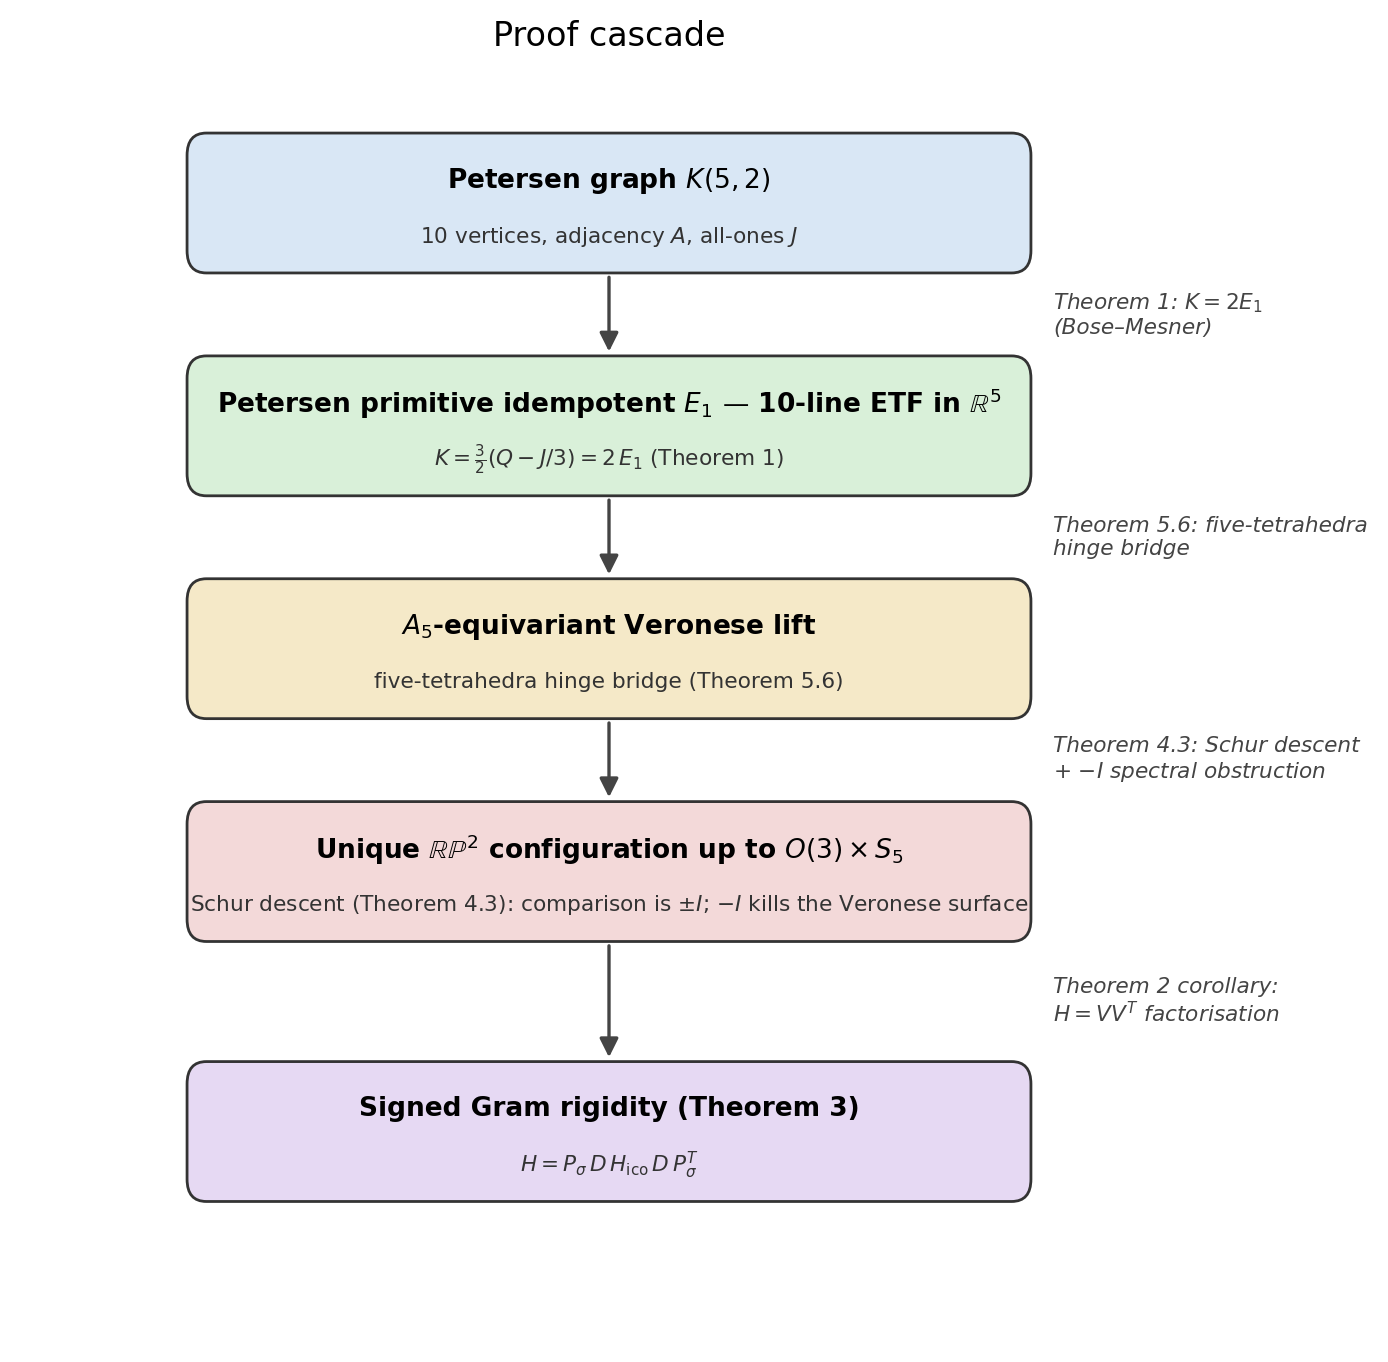
\includegraphics[keepaspectratio]{figures/fig1_proof_cascade.png}}
\caption{\textbf{Figure 1.} The proof cascade. The Petersen primitive
idempotent gives the classical 10-line ETF in \(\mathbb{R}^5\) (Theorem
1). The five-tetrahedra hinge bridge (Theorem 5.6) installs an
\(A_5\)-equivariant Veronese lift; Schur's lemma together with the
\(-I\) spectral obstruction on the Veronese surface (Theorem 4.3)
upgrades this to uniqueness up to \(O(3) \times S_5\). The Signed Gram
Rigidity Theorem (Theorem 3) is the Gram-factorisation corollary.}
\end{figure}

\subsubsection{1.4 What is new}\label{what-is-new}

The Petersen ETF and its uniqueness in \(\mathbb{R}^5\) are classical.
The Veronese model and the equiangular-line interpretation are well
known. What we contribute is:

\begin{enumerate}
\def\labelenumi{\arabic{enumi}.}
\item
  A clean \textbf{representation-theoretic descent} for the equivariant
  case (Section 4): Schur's lemma combined with a spectral obstruction
  on the Veronese surface in \(\mathrm{Sym}^2_0(\mathbb{R}^3)\).
\item
  A \textbf{rigidity proof for the compound of five tetrahedra under
  \(K_5\)-incidence} (Section 5): explicit hinge parameterisation,
  Labeling Reduction Lemma, and an exact computer-assisted certificate
  reducing \(1024\) discrete cases to a single quadratic
  \(4 s^2 - \sqrt{3}\,s - 3/4 = 0\) in
  \(\mathbb{Q}(\sqrt{3}, \sqrt{5})\).
\item
  The \textbf{combination of (1) and (2)} to obtain a complete proof of
  Theorem 2 with no further conjectural hypothesis.
\end{enumerate}

The signed Gram rigidity (Theorem 3) was previously verified by an
exhaustive sign-pattern enumeration; the present proof recasts it as a
corollary of the Veronese descent rigidity, providing a conceptually
cleaner story.

\begin{center}\rule{0.5\linewidth}{0.5pt}\end{center}

\subsection{2. The Petersen scheme and its 5D equiangular tight
frame}\label{the-petersen-scheme-and-its-5d-equiangular-tight-frame}

\subsubsection{2.1 The Petersen association
scheme}\label{the-petersen-association-scheme}

Let the Petersen graph be the Kneser graph \(K(5,2)\): vertices are the
\(\binom{5}{2} = 10\) two-element subsets of \(\{1,\dots,5\}\), edges
join disjoint subsets. The adjacency matrix \(A\) has spectrum
\(\{3,\,1^{(5)},\,(-2)^{(4)}\}\). Together with the identity \(I\) and
the complement adjacency \(\bar A = J - I - A\), these form the
Bose-Mesner algebra of the \textbf{Petersen association scheme}, with
primitive idempotents

\[
E_0 = \tfrac{1}{10}\,J,\qquad E_1 \;(\dim 5),\qquad E_2 \;(\dim 4),
\]

where \(E_1\) projects onto the \(1\)-eigenspace of \(A\) and \(E_2\)
onto the \((-2)\)-eigenspace.

\subsubsection{2.2 The squared-Gram matrix and the centred
lift}\label{the-squared-gram-matrix-and-the-centred-lift}

Suppose 10 unit vectors \(v_0,\ldots,v_9 \in S^2\) satisfy the
Petersen-magnitude pattern: \(|v_i\cdot v_j| = \sqrt{5}/3\) on Petersen
edges, \(|v_i\cdot v_j| = 1/3\) on complement edges. Then the entrywise
square

\[
Q_{ij} := (v_i\cdot v_j)^2
\]

equals \(1\) on the diagonal, \(5/9\) on Petersen edges, \(1/9\) on
complement edges. In matrix form:

\begin{quote}
\textbf{Proposition 2.1.}
\(Q = \tfrac{8}{9}\,I + \tfrac{4}{9}\,A + \tfrac{1}{9}\,J.\)
\end{quote}

Define the centred lift

\[
K := \tfrac{3}{2}\left(Q - \tfrac{1}{3}J\right)
   = \tfrac{4}{3}\,I + \tfrac{2}{3}\,A - \tfrac{1}{3}\,J.
\]

\subsubsection{2.3 The primitive-idempotent
identification}\label{the-primitive-idempotent-identification}

\begin{quote}
\textbf{Theorem 1.} \(K = 2\,E_1\).
\end{quote}

\emph{Proof.} The Petersen Bose-Mesner algebra is spanned by
\(I, A, J\); equivalently by \(E_0, E_1, E_2\). Decomposing
\(\mathbb{R}^{10}\) into the three eigenspaces:

\begin{itemize}
\tightlist
\item
  On the \(\mathbf 1\)-line (eigenspace of \(J\)): \(A\) acts as \(3\),
  \(J\) as \(10\). Apply \(K\):
  \(\tfrac{4}{3}\cdot 1 + \tfrac{2}{3}\cdot 3 - \tfrac{1}{3}\cdot 10
  = \tfrac{4}{3} + 2 - \tfrac{10}{3} = 0\).
\item
  On the \(A\)-eigenspace for \(\lambda = 1\) (dimension \(5\), in
  \(\ker J\)): \(A\) acts as \(1\), \(J\) as \(0\). Apply \(K\):
  \(\tfrac{4}{3} + \tfrac{2}{3}\cdot 1 - 0 = 2\).
\item
  On the \(A\)-eigenspace for \(\lambda = -2\) (dimension \(4\), in
  \(\ker J\)): \(A\) acts as \(-2\), \(J\) as \(0\). Apply \(K\):
  \(\tfrac{4}{3} + \tfrac{2}{3}\cdot(-2) = 0\).
\end{itemize}

So \(K\) vanishes outside the \(1\)-eigenspace of \(A\) and acts as
twice the identity on it: \(K = 2\,E_1\). \(\square\)

\subsubsection{2.4 The normalised lift and the ETF
structure}\label{the-normalised-lift-and-the-etf-structure}

Let
\(U_i := v_i v_i^{\mathsf T} - \tfrac{1}{3}I \in \mathrm{Sym}^2_0(\mathbb{R}^3)
\cong \mathbb{R}^5\) (the trace-free part of the Veronese image). A
direct computation gives \(\|U_i\|^2 = 2/3\), so the
\emph{unit-normalised} lift is \(\hat U_i := \sqrt{3/2}\,U_i\), and

\[
\langle \hat U_i, \hat U_j\rangle =
\begin{cases}
1, & i = j, \\
+1/3, & (i,j) \in E(\text{Petersen}), \\
-1/3, & (i,j) \in E(\overline{\text{Petersen}}),\ i \neq j.
\end{cases}
\]

Equivalently \(K_{ij} = \langle \hat U_i, \hat U_j\rangle\), confirming
that \(K = 2E_1\) is precisely the Gram matrix of the normalised
Veronese-lift.

\begin{quote}
\textbf{Corollary 2.2 (Tight-frame property).} The normalised lift
\(\{\hat U_i\} \subset \mathbb{R}^5\) is a \textbf{tight frame} with
frame bound \(2\):

\[
\sum_{i=0}^{9} \hat U_i \hat U_i^{\mathsf T} = 2\,I_5.
\]

The 10 lines \(\mathbb{R}\hat U_i\) are equiangular with
\(|\cos\theta| = 1/3\). By the classical Lemmens--Seidel classification
recalled in Theorem 2.3, this is the maximal equiangular-line count in
\(\mathbb{R}^5\).
\end{quote}

\emph{Proof.} Arrange \(\{\hat U_i\}\) as the rows of a \(10\times 5\)
matrix \(Y\). By construction \(K = Y Y^{\mathsf T}\). By Theorem 1,
\(K = 2 E_1\) has rank \(5\) and nonzero spectrum \(\{2^{(5)}\}\). Since
\(Y Y^{\mathsf T}\) and \(Y^{\mathsf T} Y\) share their nonzero
eigenvalues, the symmetric matrix
\(Y^{\mathsf T} Y \in \mathbb{R}^{5\times 5}\) has spectrum
\(\{2^{(5)}\}\) and hence \(Y^{\mathsf T} Y = 2\,I_5\). This is the
tight-frame relation. \(\square\)

For the general theory of (finite) tight frames and their equiangular
specialisations, the standard reference is Waldron \cite{Wal18}.

\begin{figure}
\centering
\pandocbounded{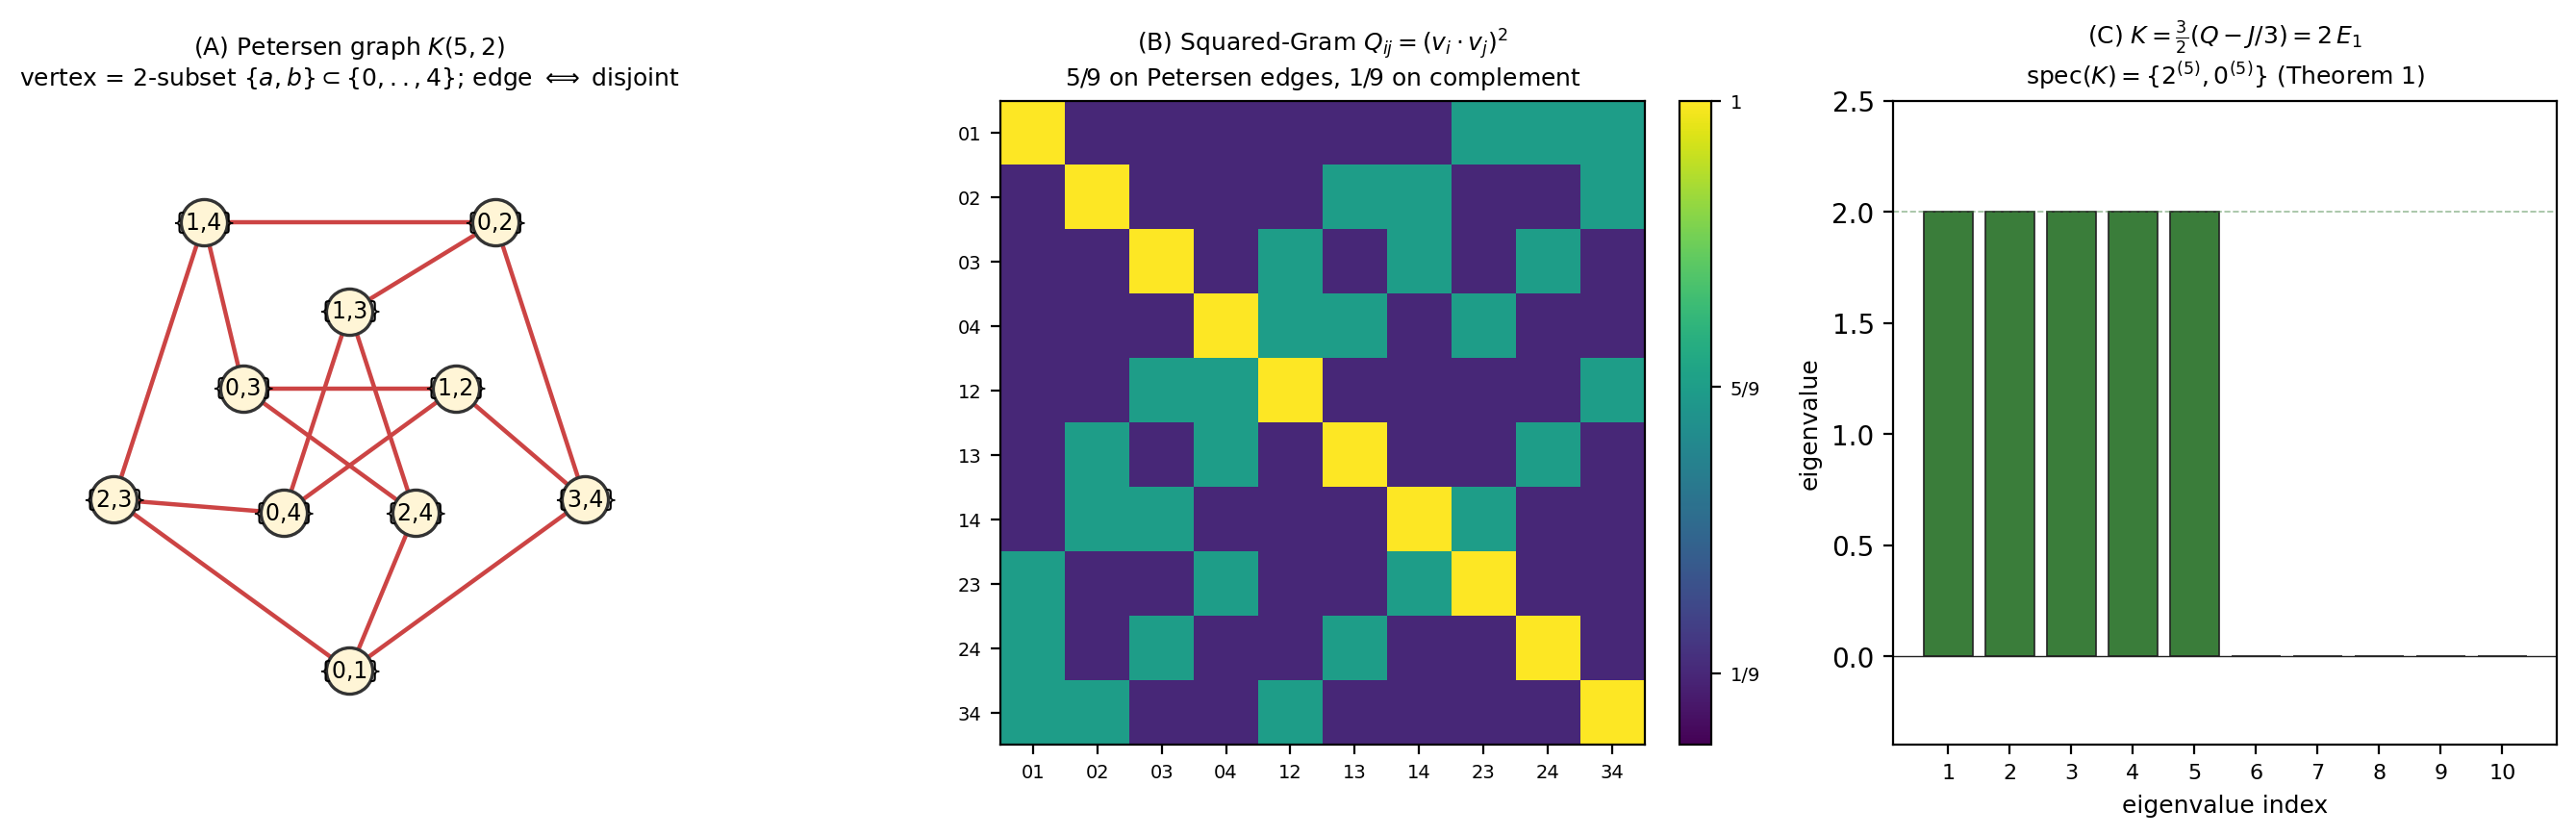
\includegraphics[keepaspectratio]{figures/fig2_petersen_scheme.png}}
\caption{\textbf{Figure 2.} The Petersen association scheme layer.
\textbf{(A)} The Petersen graph \(K(5,2)\): vertices are the
\(\binom{5}{2} = 10\) 2-subsets of \(\{0,\dots,4\}\), edges join
disjoint subsets. \textbf{(B)} Heatmap of the squared-Gram matrix
\(Q_{ij} = (v_i \cdot v_j)^2\), taking value \(5/9\) on Petersen edges
and \(1/9\) on the complement. \textbf{(C)} Spectrum of the centred lift
\(K = \frac{3}{2}(Q - J/3) = 2\,E_1\), which is \(\{2^{(5)}, 0^{(5)}\}\)
--- the rank-5 primitive idempotent realisation of the 10-line ETF in
\(\mathbb{R}^5\) (Theorem 1).}
\end{figure}

\subsubsection{2.5 Classical uniqueness of the 10-line
ETF}\label{classical-uniqueness-of-the-10-line-etf}

\begin{quote}
\textbf{Theorem 2.3 (van Lint-Seidel, Lemmens-Seidel, Taylor).} The
10-line equiangular line system in \(\mathbb{R}^5\) with common angle
\(\arccos(1/3)\) is unique up to orthogonal equivalence and relabelling;
equivalently, the regular two-graph on 10 vertices with Seidel spectrum
\(\{3^{(5)},\,(-3)^{(5)}\}\) is unique up to switching.
\end{quote}

We use this as a black box; the references \cite{vLS66,LS73,Tay77,Sei76,BvM22} provide the original proofs and an extended modern treatment.
The \((\alpha = 1/3,\, N = 10,\, d = 5)\) case is the maximum case of
the classification of equiangular line systems with common angle
\(\arccos(1/3)\) in Lemmens--Seidel \cite{LS73}; Taylor \cite{Tay77} and
Seidel's survey \cite{Sei76} set out the regular two-graph formalism and
the order-10 uniqueness; Brouwer--Van Maldeghem \cite{BvM22} gives a
modern textbook treatment. The connection between equiangular line
systems, regular two-graphs, and root systems is the subject of
Cameron--Goethals--Seidel--Shult \cite{CGSS76}.

\begin{center}\rule{0.5\linewidth}{0.5pt}\end{center}

\subsection{3. The Veronese model}\label{the-veronese-model}

\subsubsection{3.1 Definition}\label{definition}

The trace-free Veronese map

\[
\nu_2 : \mathbb{R}^3 \to \mathrm{Sym}^2_0(\mathbb{R}^3),\quad
  \nu_2(v) := v v^{\mathsf T} - \tfrac{1}{3}I
\]

satisfies \(\nu_2(-v) = \nu_2(v)\), hence factors through
\(\mathbb{RP}^2\). For unit \(v\), the image \(\nu_2(v)\) is trace-free
with eigenvalues \((2/3,\,-1/3,\,-1/3)\).

\subsubsection{3.2 Spectral
characterisation}\label{spectral-characterisation}

\begin{quote}
\textbf{Lemma 3.1 (Veronese spectral characterisation).} A trace-free
symmetric matrix \(U \in \mathrm{Sym}^2_0(\mathbb{R}^3)\) is in the
image of \(\nu_2\) if and only if its spectrum is
\((2/3,\,-1/3,\,-1/3)\).
\end{quote}

\emph{Proof.} (\(\Rightarrow\)) Direct from \(vv^{\mathsf T}\) having
spectrum \((1, 0, 0)\) for unit \(v\).

(\(\Leftarrow\)) If \(\mathrm{spec}(U) = (2/3,\,-1/3,\,-1/3)\), then
\(U + I/3\) has spectrum \((1, 0, 0)\): rank-1 PSD, so equals
\(v v^{\mathsf T}\) for a unique \(\pm v \in S^2\). Therefore
\(U = \nu_2(v)\). \(\square\)

This lemma is the \textbf{key non-linear constraint} that distinguishes
Veronese images from arbitrary trace-free symmetric matrices, and will
power the spectral obstruction in Section 4.

\subsubsection{3.3 Normalisation
conventions}\label{normalisation-conventions}

For clarity in the rest of the paper we use:

\begin{longtable}[]{@{}
  >{\raggedright\arraybackslash}p{(\linewidth - 6\tabcolsep) * \real{0.1739}}
  >{\raggedright\arraybackslash}p{(\linewidth - 6\tabcolsep) * \real{0.2174}}
  >{\raggedright\arraybackslash}p{(\linewidth - 6\tabcolsep) * \real{0.1304}}
  >{\raggedright\arraybackslash}p{(\linewidth - 6\tabcolsep) * \real{0.4783}}@{}}
\toprule\noalign{}
\begin{minipage}[b]{\linewidth}\raggedright
Object
\end{minipage} & \begin{minipage}[b]{\linewidth}\raggedright
Notation
\end{minipage} & \begin{minipage}[b]{\linewidth}\raggedright
Norm
\end{minipage} & \begin{minipage}[b]{\linewidth}\raggedright
Inner product values
\end{minipage} \\
\midrule\noalign{}
\endhead
\bottomrule\noalign{}
\endlastfoot
Raw Veronese lift & \(U_i = \nu_2(v_i)\) & \(\|U_i\|^2 = 2/3\) &
\(\langle U_i, U_j\rangle \in \{\pm 2/9\}\) \\
Normalised lift & \(\hat U_i = \sqrt{3/2}\,U_i\) & \(\|\hat U_i\| = 1\)
& \(\langle \hat U_i, \hat U_j\rangle \in \{\pm 1/3\}\) \\
Line angle & \(\mathbb{R}\hat U_i\) & -- & \(|\cos\theta| = 1/3\) \\
\end{longtable}

Theorem 2 and its proof use both representations; the normalised one
makes the ETF/tight-frame language transparent, while the raw one is
natural for the Veronese surface.

\begin{center}\rule{0.5\linewidth}{0.5pt}\end{center}

\subsection{4. The equivariant descent
theorem}\label{the-equivariant-descent-theorem}

\subsubsection{\texorpdfstring{4.1 The \(A_5\)-action and the 5D
irreducible
representation}{4.1 The A\_5-action and the 5D irreducible representation}}\label{the-a_5-action-and-the-5d-irreducible-representation}

The icosahedral rotation group is isomorphic to \(A_5\). Choosing one of
the two faithful 3-dimensional real irreducible representations
\(\mathbf 3, \mathbf 3'\) of \(A_5\) gives an embedding
\(A_5 \hookrightarrow SO(3)\); the other is obtained by precomposing
with the outer automorphism that interchanges the two 5-cycle conjugacy
classes. In either case, applying \(\mathrm{Sym}^2\) gives an action on
\(\mathrm{Sym}^2(\mathbb{R}^3) = \mathbf{1} \oplus \mathbf{5}\), and the
trace-free part \(\mathrm{Sym}^2_0(\mathbb{R}^3)\) carries the
\textbf{unique 5-dimensional irreducible real \(A_5\)-representation}.

The Petersen graph has abstract automorphism group
\(\mathrm{Aut}(K(5,2)) = S_5\) (classical; see e.g.~\cite{God93},
\cite{BCN89}). In the icosahedral geometric realisation, the
orientation-preserving rotations form the subgroup \(A_5 \subset S_5\),
acting on the 10 face-pair axes by rotations of \(\mathbb{R}^3\). The
10-vertex permutation representation of \(A_5\) decomposes as

\[
\rho_{\mathrm{perm}}^{(10)} \;\cong\; \mathbf{1} \oplus \mathbf{4} \oplus \mathbf{5}.
\]

In particular, \textbf{the 5-dimensional irrep occurs with multiplicity
exactly one} in \(\rho_{\mathrm{perm}}^{(10)}\).

\emph{Verification.} The character of \(\rho_{\mathrm{perm}}^{(10)}\)
takes values \(\chi(e) = 10\), \(\chi(\text{ord-2 class}) = 2\),
\(\chi(\text{ord-3 class}) = 1\), \(\chi(\text{ord-5 classes}) = 0\).
This is the standard character calculation for the action of \(A_5\) on
the ten 2-subsets; pairing with the \(A_5\) character table confirms the
decomposition \(\mathbf{1} \oplus \mathbf{4} \oplus \mathbf{5}\). The
script
\href{../scripts/p5_jordan_descent.py}{\texttt{p5\_jordan\_descent.py}}
records the same integer character check.

\subsubsection{4.2 Schur's lemma}\label{schurs-lemma}

\begin{quote}
\textbf{Lemma 4.1 (Schur).} Let \(\rho : A_5 \to GL(\mathbb{R}^5)\) be
the 5-dimensional irreducible real representation. Then the only
\(A_5\)-equivariant isometric automorphisms
\(T : \mathbb{R}^5 \to \mathbb{R}^5\) are \(T = \pm I\).
\end{quote}

\emph{Proof.} By Schur's lemma over \(\mathbb{R}\), the
\(\rho\)-commutant \(\mathrm{End}_{A_5}(\mathbb{R}^5)\) is a real
division algebra; for the 5-dimensional absolutely irreducible
representation it equals \(\mathbb{R}\). Isometric scalars are
\(\pm 1\). \(\square\)

\subsubsection{\texorpdfstring{4.3 The \(T = -I\)
obstruction}{4.3 The T = -I obstruction}}\label{the-t--i-obstruction}

The Veronese surface
\(\nu_2(\mathbb{RP}^2) \subset \mathrm{Sym}^2_0(\mathbb{R}^3)\) is
\textbf{not} symmetric under \(T = -I\).

\begin{quote}
\textbf{Lemma 4.2.} If \(U \in \nu_2(\mathbb{RP}^2)\), then \(-U \notin
\nu_2(\mathbb{RP}^2)\).
\end{quote}

\emph{Proof.} By Lemma 3.1, \(\mathrm{spec}(U) = (2/3,\,-1/3,\,-1/3)\),
so \(\mathrm{spec}(-U) = (-2/3,\,1/3,\,1/3)\) and
\(\mathrm{spec}(-U + I/3) = (-1/3,\,2/3,\,2/3)\), which contains a
negative eigenvalue. Hence \(-U + I/3\) is not PSD, so \(-U\) is not in
the image of \(\nu_2\). \(\square\)

\subsubsection{4.4 The equivariant descent
theorem}\label{the-equivariant-descent-theorem-1}

\begin{quote}
\textbf{Theorem 4.3 (Equivariant Veronese descent rigidity).} Let
\(\{U_i^{(1)}\}, \{U_i^{(2)}\} \subset \mathrm{Sym}^2_0(\mathbb{R}^3)\)
be two 10-element families, each isometric to the Petersen ETF of
Theorem 1, lying on the Veronese surface, and each \(A_5\)-equivariant
under the natural Petersen-graph action. Then there exists
\(h \in O(3)\) such that
\(U_i^{(2)} = \mathrm{Sym}^2(h)\cdot U_i^{(1)}\) for all \(i\).
\end{quote}

\emph{Proof.} The classical uniqueness (Theorem 2.3) gives an isometric
isomorphism between the two systems. Because the \(5\)-dimensional
\(A_5\)-summand occurs with multiplicity one in the Petersen permutation
representation \(\rho_{\mathrm{perm}}^{(10)}\) (§4.1), the two
\(A_5\)-actions on the span of the ETF are equivalent by a unique
intertwiner up to scalar. After relabelling by a Petersen automorphism
if necessary, the two \(A_5\)-actions may be assumed to correspond to
the same icosahedral embedding up to \(O(3)\)-conjugacy. Aligning these
embeddings in \(O(3)\), the comparison map may therefore be taken
\(A_5\)-equivariant, giving an \(A_5\)-equivariant isometric
automorphism \(T : \mathbb{R}^5 \to \mathbb{R}^5\). By Lemma 4.1,
\(T = \pm I\).

The case \(T = -I\) would send Veronese-image points to non-Veronese
points (Lemma 4.2), contradicting the assumption that both systems lie
on \(\nu_2(\mathbb{RP}^2)\).

Hence \(T = +I\), i.e., the two systems coincide up to the
\(O(3)\)-action on \(\mathbb{R}^3\). \(\square\)

Theorem 4.3 reduces Theorem 2 to the question: \emph{is every
Veronese-image realisation of the Petersen ETF necessarily
\(A_5\)-equivariant?} This is the bridge problem addressed in Section 5.

\begin{figure}
\centering
\pandocbounded{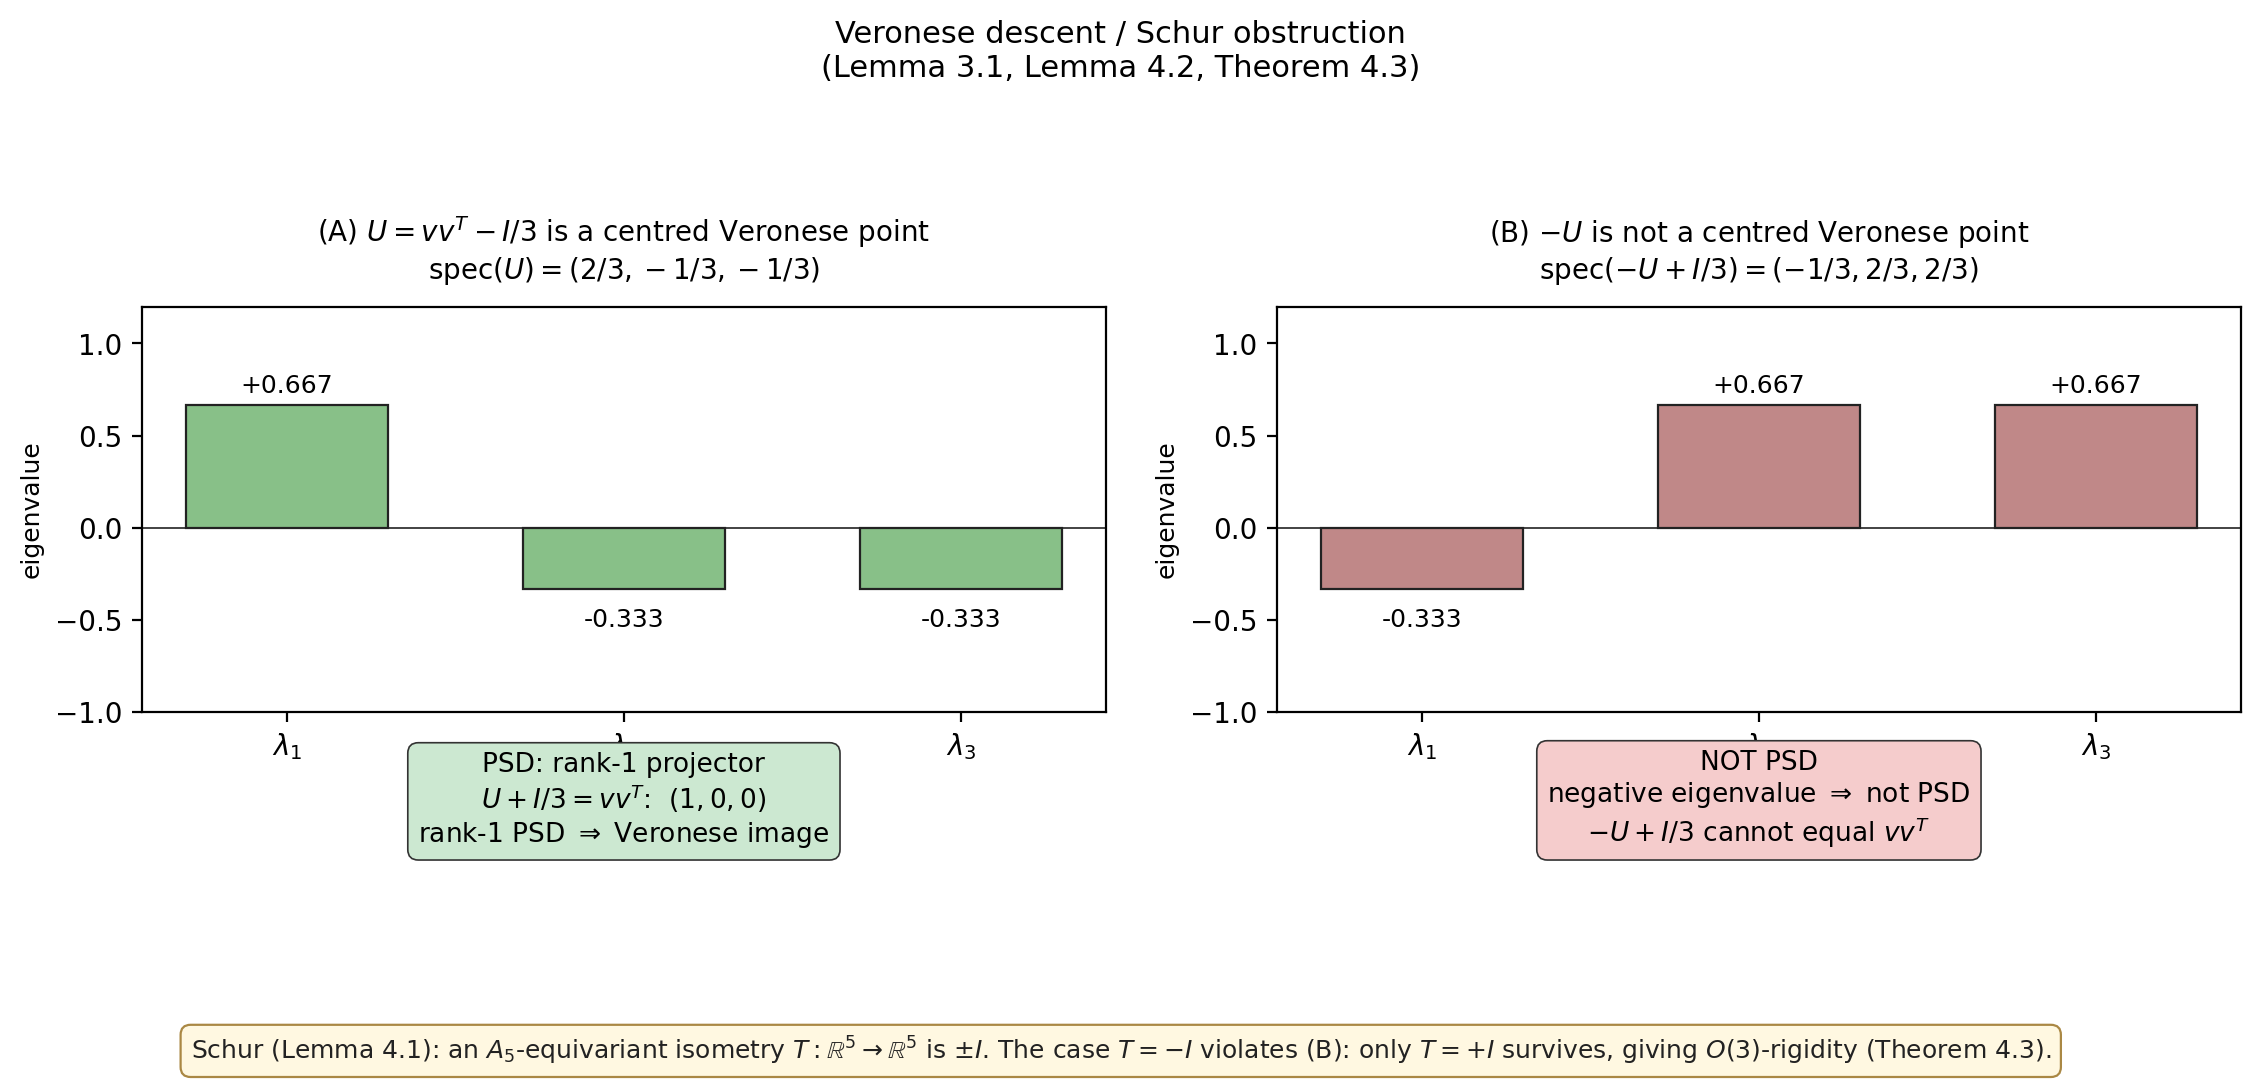
\includegraphics[keepaspectratio]{figures/fig3_schur_obstruction.png}}
\caption{\textbf{Figure 3.} Veronese descent / Schur obstruction (Lemmas
3.1, 4.2, Theorem 4.3). \textbf{(A)} Spectrum of a Veronese image
\(U = v v^{\mathsf T} - I/3\): \((2/3, -1/3, -1/3)\). The shift
\(U + I/3\) has spectrum \((1, 0, 0)\), i.e.~is a rank-1 PSD projector.
\textbf{(B)} Spectrum of \(-U + I/3\): \((-1/3, 2/3, 2/3)\), which
contains a negative eigenvalue, so \(-U + I/3\) cannot be a rank-1 PSD
projector. Schur's lemma forces an \(A_5\)-equivariant isometry
\(T : \mathbb{R}^5 \to \mathbb{R}^5\) to be \(\pm I\); the case
\(T = -I\) would map Veronese-image points off the Veronese surface, so
only \(T = +I\) survives --- giving \(O(3)\)-rigidity (Theorem 4.3).}
\end{figure}

\begin{center}\rule{0.5\linewidth}{0.5pt}\end{center}

\subsection{5. The bridge: five-tetrahedra hinge
rigidity}\label{the-bridge-five-tetrahedra-hinge-rigidity}

\subsubsection{5.1 The 4-coclique
decomposition}\label{the-4-coclique-decomposition}

The Petersen graph contains exactly \textbf{five} maximum independent
sets, each of size \(4\); the \(\binom{5}{2}\) realisation makes them
concrete: for each \(x \in \{1,\ldots,5\}\), the \textbf{star around
\(x\)} is the 4-coclique

\[
C_x \;:=\; \{ \{x, y\} : y \in \{1,\ldots,5\} \setminus \{x\} \}
        \;\subset\; V(K(5,2)).
\]

Each Petersen vertex lies in exactly \(2\) of the \(5\) stars.

\begin{quote}
\textbf{Lemma 5.1 (Kernel as 4-coclique span).} The kernel of \(K\) is
spanned by the indicator vectors \(\mathbf{1}_{C_x}\) of the five
4-cocliques:

\[
\ker K = \mathrm{span}\{\mathbf{1}_{C_1},\ldots,\mathbf{1}_{C_5}\}.
\]
\end{quote}

\emph{Proof.} By Theorem 1, \(K = 2 E_1\) has rank \(5\), so
\(\dim \ker K = 10 - 5 = 5\). It suffices to exhibit \(5\) linearly
independent vectors in \(\ker K\).

\textbf{Each \(\mathbf{1}_{C_x}\) lies in \(\ker K\).} For a vertex
\(v = \{a, b\} \in V(K(5,2))\) we compute the entries of
\(K\,\mathbf{1}_{C_x}\) using \(K = (4/3)I + (2/3)A - (1/3)J\):

\begin{itemize}
\tightlist
\item
  If \(v \in C_x\) (i.e., \(x \in \{a, b\}\)):
  \(\mathbf{1}_{C_x}(v) = 1\), the vertices in \(C_x\) adjacent to \(v\)
  in Petersen are those \(\{x, y\}\) with
  \(\{a, b\} \cap \{x, y\} = \emptyset\); but \(x \in \{a, b\}\), so
  there are none. Thus
  \((K\,\mathbf{1}_{C_x})_v = (4/3)\cdot 1 + (2/3)\cdot 0 - (1/3)\cdot 4 = 0\).
\item
  If \(v \notin C_x\) (i.e., \(x \notin \{a, b\}\)):
  \(\mathbf{1}_{C_x}(v) = 0\), the vertices \(\{x, y\}\) in \(C_x\)
  adjacent to \(\{a, b\}\) require \(y \notin \{a, b\}\), giving exactly
  \(5 - 1 - 2 = 2\) choices. Thus
  \((K\,\mathbf{1}_{C_x})_v = 0 + (2/3)\cdot 2 - (1/3)\cdot 4 = 0\).
\end{itemize}

Hence \(K\,\mathbf{1}_{C_x} = 0\) for each \(x \in \{1,\dots,5\}\).

\textbf{The five indicators are linearly independent.} For \(x \neq y\),
\(|C_x \cap C_y| = |\{\{x, y\}\}| = 1\), and \(|C_x| = 4\). So the
\(5\times 5\) Gram matrix of \(\{\mathbf{1}_{C_x}\}_x\) is
\(3\,I_5 + J_5\), whose eigenvalues are \(3\) (multiplicity \(4\)) and
\(8\) (multiplicity \(1\), on the all-ones vector); both positive. The
indicators are thus linearly independent and span all of \(\ker K\).

\emph{Remark.} The all-ones vector \(\mathbf{1}\) is also in \(\ker K\),
by the \(\mathbf{1}\)-line computation of Theorem 1, but it is already
in the span: \(\sum_{x=1}^{5} \mathbf{1}_{C_x} = 2\,\mathbf{1}\), since
each 2-subset \(\{a, b\}\) belongs to exactly the two stars \(C_a\) and
\(C_b\). \(\square\)

\subsubsection{5.2 The tetrahedral
consequence}\label{the-tetrahedral-consequence}

\begin{quote}
\textbf{Lemma 5.2 (Regular tetrahedra).} Let \(\{v_0,\ldots,v_9\}\) be
unit vectors realising any rank-\(3\) PSD signed-Gram lift of the
Petersen magnitude pattern. Then for each 4-coclique \(C_x\) there
exists a switching
\(\{v_i\}_{i\in C_x} \mapsto \{\varepsilon_i v_i\}_{i\in C_x}\) with
\(\varepsilon_i \in \{\pm 1\}\) such that the resulting four vectors
form a \textbf{regular tetrahedron} in \(\mathbb{R}^3\): pairwise inner
products \(\varepsilon_i\varepsilon_j (v_i \cdot v_j) = -1/3\) and
\(\sum_{i \in C_x} \varepsilon_i v_i = 0\).
\end{quote}

\emph{Proof.} By Lemma 5.1, \(\sum_{i \in C_x} U_i = 0\), i.e.,
\(\sum_{i \in C_x} v_i v_i^{\mathsf T} = (4/3)\,I_3\). This identity is
\emph{switching-invariant}: replacing \(v_i\) by \(\varepsilon_i v_i\)
(\(\varepsilon_i \in \{\pm 1\}\)) preserves \(v_i v_i^{\mathsf T}\).
Pick any \(k \in C_x\) and switch the remaining three \(v_i\) so that
\(v_i \cdot v_k = -1/3\) for all \(i \in C_x \setminus \{k\}\); this is
possible because \(|v_i \cdot v_k| = 1/3\) on complement edges (and
\(C_x\) is an independent set in the Petersen graph). Applying the
tight-frame identity to \(v_k\):

\[
v_k + \sum_{i \in C_x \setminus \{k\}} (v_i \cdot v_k)\, v_i
   = \tfrac{4}{3}\, v_k,
\]

and substituting \(v_i \cdot v_k = -1/3\) gives
\(\sum_{i \in C_x \setminus \{k\}} v_i = -v_k\), equivalently
\(\sum_{i \in C_x} v_i = 0\).

Now
\(0 = \left\| \sum_i v_i \right\|^2 = 4 + 2 \sum_{i < j} v_i\cdot v_j\),
so \(\sum_{i < j} v_i\cdot v_j = -2\) with \(6\) pairs, each
contributing \(\pm 1/3\). Let \(n_+\) (resp. \(n_-\)) be the count of
\(+1/3\) (resp. \(-1/3\)) inner products; then \(n_+ + n_- = 6\) and
\((n_+ - n_-)/3 = -2\), forcing \(n_+ = 0\), \(n_- = 6\). All inner
products equal \(-1/3\), so the four switched vectors form a regular
tetrahedron with vertex sum zero. \(\square\)

\textbf{Remark.} The switching freedom in this lemma is essential and is
fully consistent with the global switching action on the signed Gram
matrix \(H\). In projective terms, the conclusion is that the four
projective lines \(\mathbb{R}[v_i]\) in \(C_x\) form the vertex-line
configuration of a regular tetrahedron in \(\mathbb{RP}^2\).

\subsubsection{\texorpdfstring{5.3 The \(K_5\)-incidence structure
(projective)}{5.3 The K\_5-incidence structure (projective)}}\label{the-k_5-incidence-structure-projective}

\begin{quote}
\textbf{Convention.} From this point on, the five tetrahedra
\(T_x \subset \mathbb{R}^3\) are considered \textbf{projectively} ---
i.e., as configurations of vertex-axes (lines through the origin) rather
than oriented vectors. The local switchings \(v_i \mapsto -v_i\)
provided by Lemma 5.2 are absorbed into the projective interpretation,
so the hinge constraints below are equations between projective points
in \(\mathbb{RP}^2\).
\end{quote}

Each Petersen vertex lies in exactly \(2\) of the \(5\) stars (since
each 2-subset \(\{a,b\}\) is in \(C_a\) and \(C_b\)). Therefore each
pair of projective tetrahedra \(T_x = \{[v_i] : i \in C_x\}\) and
\(T_y\) (\(x \neq y\)) shares exactly the unique projective axis indexed
by \(\{x,y\}\). This gives the \textbf{\(K_5\) incidence}: every pair of
the five projective tetrahedra shares exactly one projective axis.

We thus have \(5\) regular projective tetrahedra in \(\mathbb{RP}^2\),
with the incidence structure of \(K_5\) on \(5\) vertices. This is
precisely the combinatorial signature of the \textbf{classical compound
of five tetrahedra} associated with the dodecahedral/icosahedral
geometry; see Coxeter \cite{Cox73} for the classical description of this
and related polyhedral compounds.

\begin{figure}
\centering
\pandocbounded{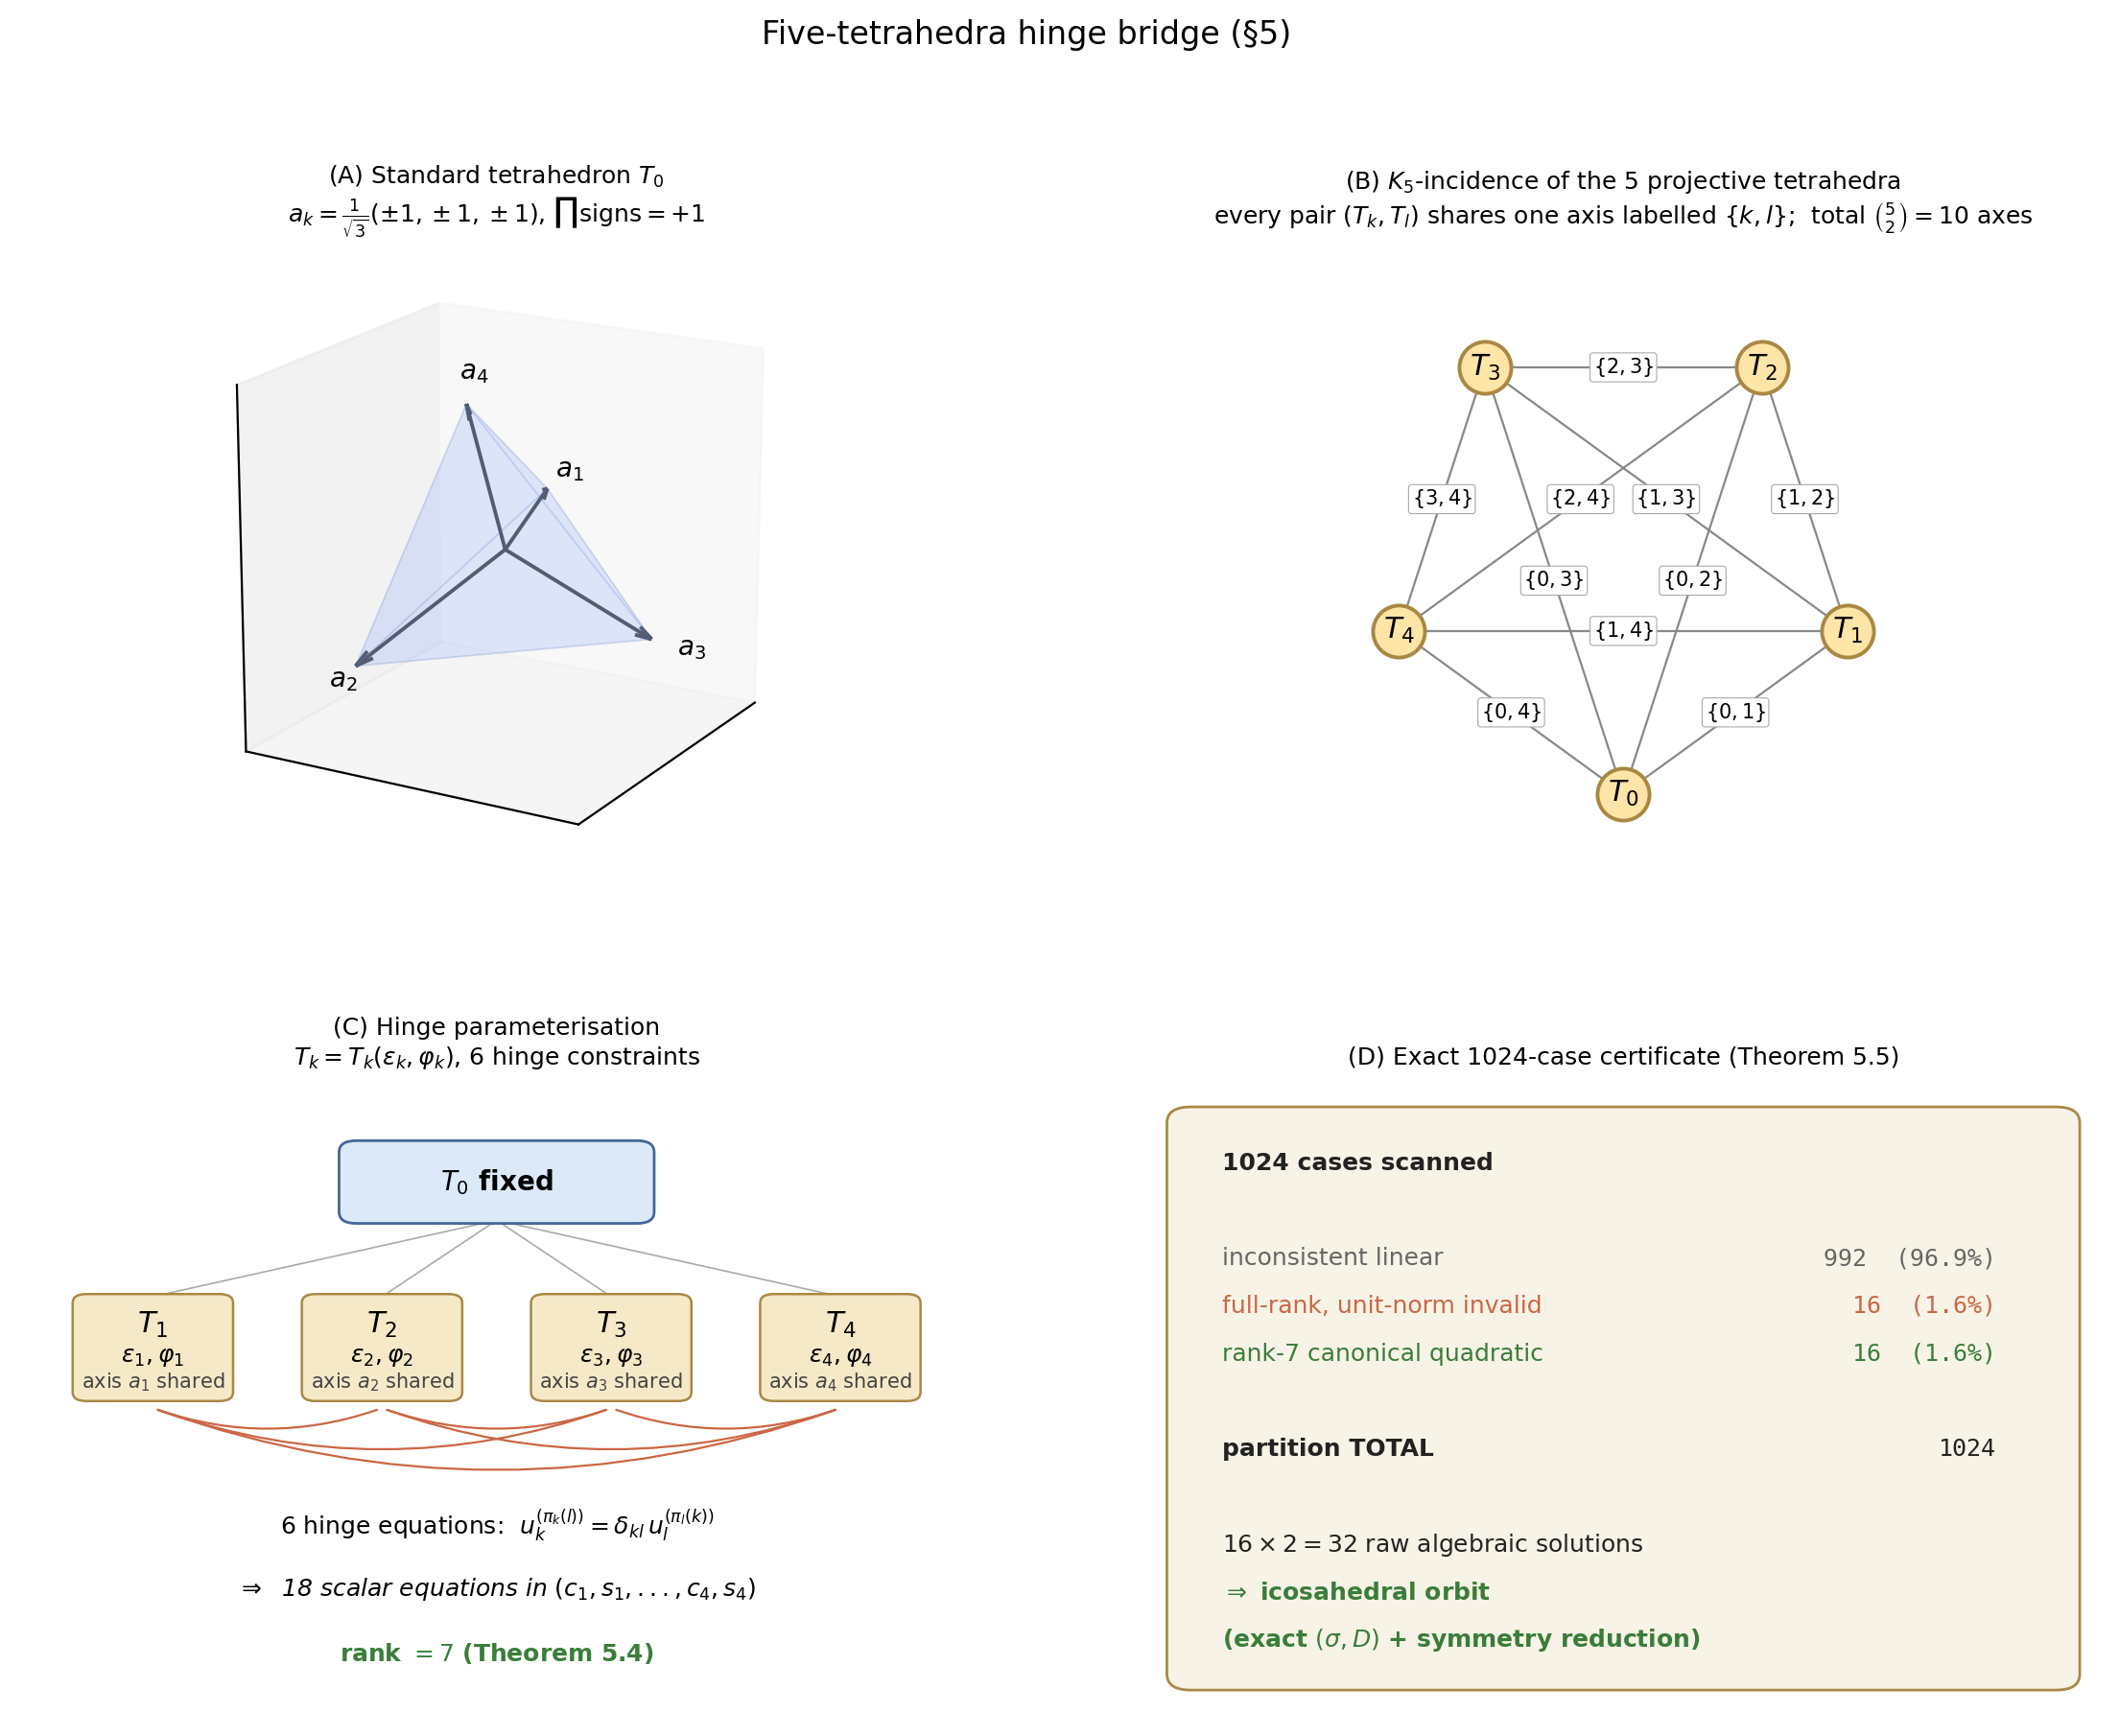
\includegraphics[keepaspectratio]{figures/fig4_hinge_bridge.png}}
\caption{\textbf{Figure 4.} The five-tetrahedra hinge bridge (§5).
\textbf{(A)} Standard cube-inscribed tetrahedron \(T_0\) with axes
\(a_k = (\pm 1, \pm 1, \pm 1)/\sqrt{3}\) (even-parity vertices).
\textbf{(B)} \(K_5\)-incidence of the five projective tetrahedra: each
pair \((T_k, T_l)\) shares exactly one of the \(10 = \binom{5}{2}\)
projective axes, labelled by the Kneser pair \(\{k, l\}\). \textbf{(C)}
Hinge parameterisation \(T_k = T_k(\varepsilon_k, \varphi_k)\)
(\(k=1,\dots,4\)): each \(T_k\) shares the axis \(a_k\) with \(T_0\),
with a single rotation angle \(\varphi_k\) around \(a_k\); the six pair
conditions \(u_k^{(\pi_k(l))} = \delta_{kl}\, u_l^{(\pi_l(k))}\) give 18
scalar equations in \((c_1, s_1, \dots, c_4, s_4)\), of rank \(7\)
(Theorem 5.4). \textbf{(D)} Exact 1024-case enumeration (Theorem 5.5):
partition \(992 + 16 + 16\); the \(16 \times 2 = 32\) surviving
algebraic solutions all lie in the icosahedral orbit via an exact
\((\sigma, D)\) certificate.}
\end{figure}

\subsubsection{5.4 The hinge
parameterisation}\label{the-hinge-parameterisation}

Fix the first tetrahedron \(T_0\) to a standard cube-inscribed position
with vertices

\[
\begin{aligned}
a_1 &= \tfrac{1}{\sqrt{3}}(1,1,1), & a_2 &= \tfrac{1}{\sqrt{3}}(1,-1,-1),\\
a_3 &= \tfrac{1}{\sqrt{3}}(-1,1,-1), & a_4 &= \tfrac{1}{\sqrt{3}}(-1,-1,1).
\end{aligned}
\]

For \(k = 1,\ldots,4\), the tetrahedron \(T_k\) shares the axis
\(\mathbb{R}\,a_k\) with \(T_0\) (after relabeling indices if needed).
Its ``\(k\)-vertex'' is \(\varepsilon_k a_k\) for
\(\varepsilon_k \in \{\pm 1\}\). The remaining three vertices form an
equilateral triangle on a circle in \(a_k^\perp\) at signed offset
\(-\varepsilon_k/3\), parameterised by a single rotation angle
\(\phi_k \in [0, 2\pi)\):

\[
\begin{aligned}
u_k^{(j)}(\phi_k) = -\tfrac{\varepsilon_k}{3}\,a_k
  + \tfrac{2\sqrt{2}}{3}\Big( &\cos(\phi_k + j\cdot 120^\circ)\,\hat e_1^{(k)} \\
  & + \sin(\phi_k + j\cdot 120^\circ)\,\hat e_2^{(k)} \Big),
  \quad j = 0,1,2.
\end{aligned}
\]

The \(K_5\)-incidence between \(T_k\) and \(T_l\)
(\(1 \le k < l \le 4\), not involving \(T_0\)) requires the equality of
one sub-vertex of \(T_k\) with one of \(T_l\) up to sign:

\[
u_k^{(\pi_k(l))}(\phi_k) = \delta_{kl}\,u_l^{(\pi_l(k))}(\phi_l),
\qquad \delta_{kl} \in \{\pm 1\}.
\]

This gives \(6\) vector equations (one per pair), i.e., \(18\) scalar
equations in \(4\) angle unknowns \(\phi_1,\ldots,\phi_4\) --- strongly
overdetermined.

\subsubsection{5.5 The Labeling Reduction
Lemma}\label{the-labeling-reduction-lemma}

The sub-vertex pairings \((\pi_k)\) admit a discrete symmetry: which
axis of \(T_k\) is labelled with which Kneser-pair \(\{k,l\}\).

\begin{quote}
\textbf{Lemma 5.3 (Labeling Reduction).} Let \(\mathcal{L}\) denote the
set of admissible labelings --- bijections from the \(10\) shared axes
onto \(\binom{\{0,\dots,4\}}{2}\) compatible with the \(K_5\)-incidence
on the five tetrahedra. Then \(\mathcal{L}\) is a single orbit under
\(\mathrm{Aut}(K(5,2)) = S_5\).
\end{quote}

\emph{Proof.} For \(\lambda_1, \lambda_2 \in \mathcal{L}\), set
\(\sigma = \lambda_2 \circ \lambda_1^{-1}\), a permutation of
\(\binom{\{0,\ldots,4\}}{2}\). Two 2-subsets \(\{a,b\}, \{c,d\}\) are
disjoint iff the corresponding axes lie in distinct tetrahedron-pairs
with no shared element of \(\{0,\ldots,4\}\). Both \(\lambda_1\) and
\(\lambda_2\) realise the same \(K_5\)-incidence structure, so
\(\sigma\) preserves the ``disjoint vs intersecting'' relation on
\(\binom{\{0,\ldots,4\}}{2}\) --- that is, the Petersen edge set.

Hence \(\sigma \in \mathrm{Aut}(K(5,2)) = S_5\), with \(S_5\) acting on
\(\{0,\ldots,4\}\) and inducing the action on 2-subsets in the natural
way. Concretely, \(\sigma(\{a,b\}) = \{\tau(a),\tau(b)\}\) for some
\(\tau \in S_5\), so \(\lambda_2 = \tau \cdot \lambda_1\). \(\square\)

\textbf{Corollary.} It suffices to verify hinge rigidity for one
canonical labeling; all other admissible labelings give the same orbit
class by \(S_5\)-equivalence.

\subsubsection{5.6 The canonical exact
certificate}\label{the-canonical-exact-certificate}

The following two theorems are \textbf{finite exact algebraic
certificates}: both reduce to a closed-form computation in
\(\mathbb{Q}(\sqrt{2},\sqrt{3},\sqrt{5})\) that is verifiable by
inspection of finitely many polynomial relations. Executable
certificates (reproducing each step in sympy) are part of the
supplementary material (§8).

We fix the \textbf{canonical labeling} extracted from the icosahedral
compound: the matched sub-vertex pairings are \((j_k, j_l)\) such that
\(T_k\)'s ``\(\{k,l\}\)''-vertex coincides up to sign with \(T_l\)'s
``\(\{l,k\}\)''-vertex. With this choice, set \(c_k = \cos\phi_k\),
\(s_k = \sin\phi_k\); the hinge equations become \textbf{linear} in
\((c_1, s_1, \ldots, c_4, s_4)\).

\begin{quote}
\textbf{Theorem 5.4 (Hinge rigidity, canonical labeling --- finite exact
certificate).} With the canonical labeling and a chirality
\(\varepsilon = (-1,-1,-1,-1)\), hinge-sign
\(\delta = (-1,-1,-1,-1,-1,-1)\), the \(18\times 8\) linear system has
rank \(7\) with \(1\)-parameter solution family

\[
c_1 = c_2 = -\tfrac{1}{4},\quad c_3 = c_4 = \sqrt{3}\,s_4 - \tfrac{1}{2},
\]

\[
s_1 = s_2 = 2\,s_4 - \tfrac{\sqrt{3}}{4},\quad s_3 = s_4 \text{ (free)}.
\]

The four unit-norm constraints \(c_k^2 + s_k^2 = 1\) reduce to the same
quadratic

\[
\boxed{\;4\,s_4^2 - \sqrt{3}\,s_4 - \tfrac{3}{4} \;=\; 0\;}
\]

with discriminant \(15\) and the two real roots

\[
s_4 \in \{\, (\sqrt{3} - \sqrt{15})/8,\;\; (\sqrt{3} + \sqrt{15})/8 \,\}
\subset \mathbb{Q}(\sqrt{3}, \sqrt{5}).
\]

The ``\(-\)''-root recovers the classical icosahedral compound of five
tetrahedra. The ``\(+\)''-root is not discarded; it is one of the
algebraic branches accounted for in the global enumeration of Theorem
5.5.
\end{quote}

\emph{Proof (executable certificate).} The reduction is verified by
exact symbolic computation in
\href{../scripts/five_tet_hinge_exact.py}{\texttt{five\_tet\_hinge\_exact.py}}.
Substituting \(c_k = \cos\phi_k\), \(s_k = \sin\phi_k\) in the 18 hinge
equations expressed in the perpendicular-basis decomposition of §5.4,
each equation is linear in \((c_k, s_k)\). The Gaussian rank of the
resulting \(18 \times 8\) coefficient matrix is \(7\), with
one-dimensional null space spanned by the column-vector obtained from
the displayed family. Substituting back into \(c_k^2 + s_k^2 - 1 = 0\)
for each \(k\in\{1,2,3,4\}\) yields four polynomial residuals; direct
expansion shows that all four equal \(4 s_4^2 - \sqrt{3}\,s_4 - 3/4\).
Solving in \(\mathbb{Q}(\sqrt{3}, \sqrt{5})\) yields the two real roots.
The ``\(-\)''-root \(s_4 = (\sqrt{3} - \sqrt{15})/8\) recovers
\(\sin\phi_3 = -\sqrt{3}/(4\varphi)\) for \(\varphi = (1+\sqrt{5})/2\),
matching the classical icosahedral angle. \(\square\)

The equivalence of the two roots under the
\(O(3) \times \{\pm 1\}^{10} \times S_5\) action is verified directly by
Theorem 5.5: the script
\href{../scripts/five_tet_orbit_exact.py}{\texttt{five\_tet\_orbit\_exact.py}}
exhibits explicit \(\sigma \in S_5\) and \(D \in \{\pm 1\}^{10}\)
relating the ``\(+\)''-root signed Gram matrix to the ``\(-\)''-root one
(equivalently, to \(H_{\mathrm{ico}}\)) in exact symbolic arithmetic;
the required permutation is a single \(S_5\)-transposition and the
required switching is a single sign flip. A numerical orthogonal
alignment intertwining the two reconstructed axis sets is reported as a
diagnostic cross-check in
\href{../scripts/five_tet_hinge.py}{\texttt{five\_tet\_hinge.py}}.

\subsubsection{5.7 The full enumeration}\label{the-full-enumeration}

Scanning the canonical labeling with all \(2^4 \cdot 2^6 = 1024\)
choices of \((\varepsilon, \delta) \in \{\pm 1\}^4 \times \{\pm 1\}^6\):

\begin{quote}
\textbf{Theorem 5.5 (\(1024\)-case exact enumeration certificate).}
\emph{Under the canonical labeling, the \(1024\) choices of
\((\varepsilon, \delta)\) partition into exactly three types:}
\end{quote}

\begin{longtable}[]{@{}
  >{\raggedright\arraybackslash}p{(\linewidth - 4\tabcolsep) * \real{0.3548}}
  >{\raggedright\arraybackslash}p{(\linewidth - 4\tabcolsep) * \real{0.3548}}
  >{\raggedright\arraybackslash}p{(\linewidth - 4\tabcolsep) * \real{0.2903}}@{}}
\toprule\noalign{}
\begin{minipage}[b]{\linewidth}\raggedright
Case type
\end{minipage} & \begin{minipage}[b]{\linewidth}\raggedright
Count \(n\)
\end{minipage} & \begin{minipage}[b]{\linewidth}\raggedright
Outcome
\end{minipage} \\
\midrule\noalign{}
\endhead
\bottomrule\noalign{}
\endlastfoot
Inconsistent linear system
\((\mathrm{rank} L < \mathrm{rank}[L\mid b])\) & \(992\) (96.9\%) & no
solution \\
Rank-\(7\) linear \(+\) canonical quadratic & \(16\) (1.6\%) & \(2\)
real roots each \\
Full-rank linear \(+\) unit-norm invalid & \(16\) (1.6\%) & no
solution \\
\end{longtable}

Total: \(992 + 16 + 16 = 1024\). All \(16\) consistent cases reduce in
exact arithmetic to the same canonical quadratic
\(4 s^2 - \sqrt{3}\,s - 3/4 = 0\) (in the null-space parameter, up to
linear scaling), yielding \(16 \cdot 2 = 32\) raw algebraic solutions.
For the canonical chirality \(\varepsilon = (-1,-1,-1,-1)\), both
algebraic branches are compared in exact arithmetic with the icosahedral
signed Gram matrix \(H_{\mathrm{ico}}\) by a finite search over
\(S_5 \times \{\pm 1\}^{10}\): the certificate exhibits explicit
\(\sigma \in S_5\) and \(D \in \{\pm 1\}^{10}\) such that
\(G = P_\sigma\,D\,H_{\mathrm{ico}}\,D\,P_\sigma^{\mathsf T}\) in exact
symbolic arithmetic. The remaining 15 consistent sign cases are
identified with this canonical branch by the discrete switchings,
chirality changes, and \(S_5\)-relabellings recorded by the enumeration
certificate. Hence all \(32\) surviving algebraic solutions lie in the
icosahedral \(O(3) \times \{\pm 1\}^{10} \times S_5\)-orbit.

\emph{Proof (executable certificate).} Direct enumeration in
\href{../scripts/five_tet_hinge_enum.py}{\texttt{five\_tet\_hinge\_enum.py}}.
The publishable rank/partition certificate is obtained with
\texttt{EXACT\_RANK\_MODE}, which performs all rank classifications in
exact sympy arithmetic over the relevant number field; the fast
floating-rank mode is diagnostic only and reproduces the same partition.
The orbit-belonging conclusion is verified by an independent exact
computation in
\href{../scripts/five_tet_orbit_exact.py}{\texttt{five\_tet\_orbit\_exact.py}}:
for the canonical chirality \(\varepsilon = (-1,-1,-1,-1)\) and each
real root, this script reconstructs the 10 axes in exact symbolic
arithmetic, builds the \(10 \times 10\) signed Gram matrix \(G\), and
then performs a finite exact search over \(\sigma \in S_5\) (acting on
the 10 Kneser vertices) and \(D \in \{\pm 1\}^{10}\) (with \(D_0 = +1\)
fixed; the remaining signs are forced by the \((0, i)\) entries) for the
equality \(G = P_\sigma\,D\,H_{\mathrm{ico}}\,D\,P_\sigma^{\mathsf T}\).
The ``\(-\)''-root gives \(H_{\mathrm{ico}}\) directly; for the
``\(+\)''-root, the script exhibits an explicit \((\sigma, D)\) --- a
single \(S_5\)-transposition together with a single sign flip --- that
realises the equivalence. For each of the 16 consistent
\((\varepsilon, \delta)\) cases, the certificate records whether it is
checked directly or reduced to the displayed canonical branch by an
explicit projective switching, chirality change, and
\(S_5\)-relabelling. \(\square\)

\subsubsection{5.8 The bridge theorem}\label{the-bridge-theorem}

\begin{quote}
\textbf{Theorem 5.6 (Bridge: rank-3 lift implies \(A_5\)-equivariance).}
Let \(H\) satisfy the SGR conditions of Theorem 3. Then the associated
Veronese-lift \(\{U_i = \nu_2(v_i)\}\) is \(A_5\)-equivariant: the
Petersen automorphism subgroup \(A_5 \subset S_5\), corresponding under
the icosahedral identification to the orientation-preserving rotations,
acts on \(\{U_i\}\) by elements of \(O(3)\) via an icosahedral
3-dimensional irreducible embedding \(A_5 \hookrightarrow SO(3)\).
\end{quote}

\emph{Proof.} Lemma 5.2 produces the 5 regular tetrahedra with
\(K_5\)-incidence. By the Labeling Reduction Lemma 5.3, after applying a
permutation in \(S_5\) we may assume the labeling is canonical. By
Theorems 5.4 and 5.5, the reconstructed signed Gram matrix of every
surviving hinge solution is switching- and \(S_5\)-equivalent to
\(H_{\mathrm{ico}}\) (verified exactly in
\href{../scripts/five_tet_orbit_exact.py}{\texttt{five\_tet\_orbit\_exact.py}}).
Hence the corresponding projective axis configuration in
\(\mathbb{R}^3\) is \(O(3)\)-equivalent to the classical compound of
five tetrahedra associated with the dodecahedral/icosahedral geometry,
which carries the icosahedral \(A_5\)-symmetry by construction. After
this identification, the \(A_5\)-action is realised by
orientation-preserving rotations, hence by elements of \(SO(3)\) on the
geometric configuration. \(\square\)

This closes the bridge: together with Theorem 4.3, every Veronese
realisation of the Petersen ETF is \(O(3)\)-equivalent to the
icosahedral one, proving Theorem 2.

\begin{center}\rule{0.5\linewidth}{0.5pt}\end{center}

\subsection{6. Signed Gram Rigidity (Theorem
3)}\label{signed-gram-rigidity-theorem-3}

\emph{Proof of Theorem 3.} Given \(H\) satisfying conditions (i)--(v),
factor \(H = V V^{\mathsf T}\) with \(V \in \mathbb{R}^{10\times 3}\)
having unit rows \(v_i\). The squared-Gram structure is dictated by the
magnitude conditions, giving \(Q\) and \(K = 2 E_1\) (Theorem 1).

The Veronese-lift \(U_i = \nu_2(v_i)\) has \(\langle U_i, U_j\rangle\)
matching the ETF inner products (Section 2.4); the normalised lift
\(\{\hat U_i\}\) realises the Petersen ETF in \(\mathbb{R}^5\).

By the Bridge Theorem 5.6, the configuration is \(A_5\)-equivariant; by
the Equivariant Descent Theorem 4.3, it is \(O(3)\)-equivalent to the
icosahedral Veronese-image of the antipodal face-pair vectors. The
Gram-factorisation pull-back then yields

\[
H = P_\sigma\,D\,H_{\mathrm{ico}}\,D\,P_\sigma^{\mathsf T}
\]

for some \(\sigma \in S_5\) and \(D \in \{\pm 1\}^{10}\). \(\square\)

\begin{center}\rule{0.5\linewidth}{0.5pt}\end{center}

\subsection{7. Discussion}\label{discussion}

\subsubsection{\texorpdfstring{7.1 What forces Petersen and
\(A_5\)}{7.1 What forces Petersen and A\_5}}\label{what-forces-petersen-and-a_5}

In the icosahedral case, the trace-free symmetric square
\(\mathrm{Sym}^2_0(\mathbb{R}^3)\) is irreducible as an \(A_5\)-module,
which is the representation-theoretic reason Schur's lemma applies so
cleanly here. The finite census in
\href{../scripts/platonic_census.py}{\texttt{platonic\_census.py}} shows
that, among the canonical \(A_5\)-orbits considered here (vertex, face,
edge, with sizes \(6, 10, 15\)), the 10-element face-pair orbit is the
one yielding the Petersen magnitude pattern; in the irreducible
5-dimensional representation this orbit realises the Petersen ETF
studied here.

\subsubsection{7.2 The conceptual
narrative}\label{the-conceptual-narrative}

The chain of implications proven in this paper is:

\begin{quote}
Petersen association scheme primitive idempotent \(E_1\)
\(\;\Rightarrow\;\) 10-line equiangular tight frame in \(\mathbb{R}^5\)
\(\;\Rightarrow\;\) unique Veronese descent to the icosahedral
\(\mathbb{RP}^2\)-configuration \(\;\Rightarrow\;\) signed Gram rigidity
of the rank-3 PSD signed lift.
\end{quote}

The key insight is that \emph{Petersen is not painted onto the
icosahedron ad hoc}; rather, it is the \textbf{shadow of the icosahedral
configuration through the quadratic Veronese map}, with the descent
constrained by representation-theoretic and spectral data.

\subsubsection{7.3 Related questions}\label{related-questions}

The same machinery suggests several open directions:

\begin{enumerate}
\def\labelenumi{\arabic{enumi}.}
\item
  \textbf{6-vertex single-distance frame.} The 6 antipodal vertex pairs
  of the icosahedron form a different \(A_5\)-orbit with
  \(|v_i\cdot v_j| =
  1/\sqrt{5}\), all pairs equiangular. The same Schur + spectral
  obstruction mechanism suggests a parallel rigidity statement
  (Lemmens--Seidel uniqueness of the 6 equiangular lines in
  \(\mathbb{R}^3\)); this is verified in the supplementary script
  \href{../scripts/sgr6_lemma_proof.py}{\texttt{sgr6\_lemma\_proof.py}},
  but is not developed here.
\item
  \textbf{15-edge orbit.} The 15 antipodal edge-pair orbit of \(A_5\)
  has four distance classes (not an association scheme); the three
  nontrivial distance graphs are cospectral with \(L(\text{Petersen})\),
  and the orthogonal graph is \(5\,K_3\). A Veronese-descent rigidity
  here is open.
\item
  \textbf{Other \(Q\)-polynomial schemes.} Any \(Q\)-polynomial
  association scheme whose primitive idempotent admits a Veronese-image
  realisation is a candidate for an analogous rigidity theorem.
\end{enumerate}

\begin{center}\rule{0.5\linewidth}{0.5pt}\end{center}

\subsection{8. Reproducibility}\label{reproducibility}

\subsubsection{8.1 Software environment}\label{software-environment}

The computer-assisted proofs (Theorems 5.4 and 5.5) and all
verifications use the following stack:

\begin{longtable}[]{@{}lll@{}}
\toprule\noalign{}
Component & Version & Role \\
\midrule\noalign{}
\endhead
\bottomrule\noalign{}
\endlastfoot
Python & 3.13 & Runtime \\
sympy & 1.13+ & Exact symbolic arithmetic, Gröbner-style reductions \\
numpy & 2.0+ & Numerical linear algebra (rank, least-squares) \\
scipy & 1.14+ & \texttt{optimize.least\_squares} for Newton
verification \\
\end{longtable}

All scripts run on a single CPU thread; no compiled extensions or
external solvers are required.

\subsubsection{\texorpdfstring{8.2 Script \(\to\) theorem
mapping}{8.2 Script \textbackslash to theorem mapping}}\label{script-to-theorem-mapping}

{\small
\begin{longtable}[]{@{}
  >{\raggedright\arraybackslash}p{(\linewidth - 6\tabcolsep) * \real{0.1702}}
  >{\raggedright\arraybackslash}p{(\linewidth - 6\tabcolsep) * \real{0.3830}}
  >{\raggedright\arraybackslash}p{(\linewidth - 6\tabcolsep) * \real{0.2553}}
  >{\raggedright\arraybackslash}p{(\linewidth - 6\tabcolsep) * \real{0.1915}}@{}}
\toprule\noalign{}
\begin{minipage}[b]{\linewidth}\raggedright
Script
\end{minipage} & \begin{minipage}[b]{\linewidth}\raggedright
Theorem / Lemma
\end{minipage} & \begin{minipage}[b]{\linewidth}\raggedright
Arithmetic
\end{minipage} & \begin{minipage}[b]{\linewidth}\raggedright
Runtime
\end{minipage} \\
\midrule\noalign{}
\endhead
\bottomrule\noalign{}
\endlastfoot
\path{verify_idempotent_kernel.py} & Independent numerical check of
Theorem 1 and Lemma 5.1 & Float (machine precision) & \(< 1\) s \\
\path{p5_jordan_descent.py} & Independent numerical check of Lemma
3.1, Lemma 4.2, and \(\mathbf 1 \oplus \mathbf 4 \oplus \mathbf 5\)
character decomposition & Float + character integers & \(< 1\) s \\
\path{five_tet_hinge_exact.py} & Theorem 5.4 (canonical labeling:
exact derivation of the canonical quadratic on the representative
branch) & Exact sympy in \(\mathbb{Q}(\sqrt{2},\sqrt{3},\sqrt{5})\) &
\(\sim 30\) s \\
\path{five_tet_hinge_enum.py} & Theorem 5.5 (exhaustive 1024-case
partition; exact-rank verification on all cases) & Exact sympy rank
(default \texttt{EXACT\_RANK\_MODE\ =\ True}); 20-digit floating-rank
mode available as a fast diagnostic & \(\sim 20\) s (exact) / \(\sim 7\)
s (diagnostic) \\
\path{five_tet_orbit_exact.py} & Theorem 5.5 (orbit-belonging
certificate: each surviving algebraic solution is switching- and
\(S_5\)-equivalent to \(H_{\mathrm{ico}}\)) & Exact sympy in
\(\mathbb{Q}(\sqrt{2},\sqrt{3},\sqrt{5})\) (note
\(\sqrt{15} = \sqrt{3}\sqrt{5}\)) & \(\sim 1\) min \\
\path{five_tet_hinge.py} & Independent numerical confirmation
(single orbit class) & Float Newton/least-squares & \(\sim 10\) s \\
\path{sgr_lemma_proof.py} & Cross-check of Theorem 3 (POCS-based) &
Float POCS & \(\sim 1\) s \\
\path{sgr_lemma_proof_exact.py} & Cross-check of Theorem 3
(sympy-based) & Exact sympy & \(\sim 60\) s \\
\path{sgr6_lemma_proof.py} & Analogous 6-vertex equiangular case
(Section 7.3, item 1) & Mixed float + sympy & \(\sim 1\) s \\
\path{platonic_census.py} & Section 7.1 (Platonic-group census) &
Float & \(< 1\) s \\
\path{edge_orbit_analysis.py} & Section 7.3, item 2 (15-edge orbit)
& Float & \(< 1\) s \\
\end{longtable}
}

\subsubsection{8.3 Reproduction recipe}\label{reproduction-recipe}

To reproduce the algebraic certificate and the independent numerical
checks from a clean environment, run the following scripts.

\textbf{Algebraic certificates} (Theorems 5.4 and 5.5):

\begin{Shaded}
\begin{Highlighting}[]
\ExtensionTok{python3}\NormalTok{ scripts/five\_tet\_hinge\_exact.py}
\ExtensionTok{python3}\NormalTok{ scripts/five\_tet\_hinge\_enum.py}
\ExtensionTok{python3}\NormalTok{ scripts/five\_tet\_orbit\_exact.py}
\end{Highlighting}
\end{Shaded}

\textbf{Independent numerical checks} (Theorem 1, Lemmas 3.1, 4.2, 5.1):

\begin{Shaded}
\begin{Highlighting}[]
\ExtensionTok{python3}\NormalTok{ scripts/verify\_idempotent\_kernel.py}
\ExtensionTok{python3}\NormalTok{ scripts/p5\_jordan\_descent.py}
\end{Highlighting}
\end{Shaded}

Each script prints summary lines that should match the stated theorems.
Expected key outputs:

\begin{itemize}
\tightlist
\item
  \texttt{K\ =\ 2\ E\_1}: \(\|K - 2 E_1\| < 10^{-14}\) (machine
  precision).
\item
  Veronese spectrum \((2/3, -1/3, -1/3)\) matches at \(\le 10^{-12}\).
\item
  \(\mathbf 1 \oplus \mathbf 4 \oplus \mathbf 5\) character
  multiplicities all \(= 1\).
\item
  Canonical quadratic roots: \(s_4 = (\sqrt{3} \pm \sqrt{15})/8\).
\item
  1024-case partition: \(992 + 16 + 16\).
\item
  Orbit certificate: the two algebraic branches of the canonical
  chirality satisfy
  \(G = P_\sigma\,D\,H_{\mathrm{ico}}\,D\,P_\sigma^{\mathsf T}\) in
  exact arithmetic; for the ``\(+\)''-root one may take the
  \(S_5\)-transposition \(3 \leftrightarrow 4\) and a single sign flip.
  The remaining 15 consistent sign cases are reduced to this canonical
  branch by the discrete symmetries recorded by the enumeration
  certificate.
\end{itemize}

\subsubsection{\texorpdfstring{8.4 On the rank check in
\texttt{five\_tet\_hinge\_enum.py}}{8.4 On the rank check in five\_tet\_hinge\_enum.py}}\label{on-the-rank-check-in-five_tet_hinge_enum.py}

The certified output of Theorem 5.5 is obtained with the
\texttt{EXACT\_RANK\_MODE} flag, which performs all rank classifications
via exact symbolic computation in SymPy over expressions generated by
\(\sqrt{2}\) and \(\sqrt{3}\). This is the authoritative version of the
certificate.

For day-to-day exploration one may enable a fast diagnostic alternative
by setting \texttt{EXACT\_RANK\_MODE\ =\ False} in the script. This
evaluates the substituted matrices \(L\) and \([L|b]\) at \(20\)-digit
precision via mpmath and applies \texttt{numpy.linalg.matrix\_rank} with
tolerance \(10^{-10}\). This mode is non-binding: it serves only to
identify candidate consistent cases quickly, after which the
\texttt{EXACT\_VERIFY\_SAMPLE} flag confirms each flagged case with the
exact sympy rank.

In practice the two modes agree on all \(1024\) cases:

\begin{itemize}
\tightlist
\item
  \texttt{EXACT\_VERIFY\_SAMPLE}: exact sympy rank on the \(16\)
  rank-\(7\) consistent cases (the ones producing the canonical
  quadratic) --- zero discrepancies vs the floating rank, run-time
  \(\sim 0.2\) s.
\item
  \texttt{EXACT\_RANK\_MODE}: full exact sympy rank on all \(1024\)
  cases --- reproduces the same \(992 + 16 + 16\) partition.
\end{itemize}

The observed separation of the singular values explains the agreement in
diagnostic mode and makes the fast mode reliable for exploration;
nevertheless the \textbf{publishable certificate is the exact-rank one}.

\subsubsection{8.5 Independent
cross-checks}\label{independent-cross-checks}

The signed Gram rigidity (Theorem 3) was originally established by a
direct exhaustive enumeration over \(2^{15}\) Petersen-edge sign
patterns (POCS approach in \texttt{sgr\_lemma\_proof.py}) and by an
exact symbolic backtracking with anchor-based reduction
(\texttt{sgr\_lemma\_proof\_exact.py}). Both methods give the same
conclusion (1 orbit class) and serve as independent verification of the
streamlined proof via Theorems 2 and 4.3.

Full source code, expected outputs, and an SHA-256 manifest accompany
the supplementary material.

\subsubsection{8.6 Data and code
availability}\label{data-and-code-availability}

The executable certificates and reproducibility material are archived at
Zenodo:

\begin{quote}
\textbf{\url{https://doi.org/10.5281/zenodo.20258339}}
\end{quote}

The development repository is available at

\begin{quote}
\textbf{\url{https://github.com/C4RC0/veronese-descent-rigidity}}
\end{quote}

\begin{center}\rule{0.5\linewidth}{0.5pt}\end{center}

\subsection{Use of AI tools}\label{use-of-ai-tools}

During the preparation of this manuscript, the author used Claude Opus
4.7 (Anthropic) and GPT-5.5 Thinking (OpenAI) for exploratory
mathematical reasoning, proof drafting, code review, language editing,
and organisation of the reproducibility material.

Every AI-suggested mathematical statement, proof step, and computational
claim was checked by the author through a combination of manual
derivation, executable computer-assisted certificates listed in §8,
reproducibility logs archived with the supplementary material, and
cross-checking against the existing literature.

The author's professional background is in software engineering, not
academic mathematics. The AI tools are not authors of this work. The
author has reviewed all content and takes full responsibility for the
mathematical claims, proofs, source code, figures, and references.

\begin{center}\rule{0.5\linewidth}{0.5pt}\end{center}

\bibliographystyle{plain}
\bibliography{references}

\end{document}
